\documentclass[journal]{IEEEtran}

\usepackage[utf8]{inputenc}
\usepackage[T1]{fontenc}
\usepackage{graphicx}
\usepackage{amsmath,amssymb}
\usepackage{booktabs}
\usepackage{multirow}
\usepackage{dcolumn}
\usepackage{xcolor}
\usepackage{float}
\usepackage{url}
\usepackage[hidelinks,bookmarksopen=true,bookmarksnumbered=true]{hyperref}

\newcolumntype{.}{D{.}{.}{-1}}
\newcolumntype{d}[1]{D{.}{.}{#1}}
\newcolumntype{e}{D{E}{E}{-1}}
\newcolumntype{E}[1]{D{E}{E}{#1}}

\newcommand{\eqnref}[1]{Eq.(\ref{#1})}

\hypersetup{
  pdftitle={Open-Vocabulary Referring Segmentation of Aerial Photos},
  pdfauthor={Luis Pedro Soares Marnoto Gaspar Lopes},
  pdfcreator={LaTeX with hyperref}
}

\begin{document}

\title{Open-Vocabulary Referring Segmentation of Aerial Photos}
\author{Luis Pedro Soares Marnoto Gaspar Lopes\thanks{INESC-ID, Instituto Superior Técnico, University of Lisbon, Lisbon, Portugal. Email: luis.marnoto.gaspar.lopes@tecnico.ulisboa.pt}}

\maketitle

\begin{abstract}
Referring expression segmentation is a fundamental task in computer vision that integrates natural language understanding with precise visual localization of target regions. Applying this to aerial imagery presents unique challenges because spatial resolution varies widely across datasets, targets often shrink to only a few pixels, and scenes contain very high object densities. This work presents Aerial-D, a large-scale referring expression segmentation dataset for aerial imagery comprising 37,288 image patches with 1,522,523 referring expressions covering 259,709 annotated targets across individual objects, groups, and semantic categories spanning 21 distinct classes from vehicles and infrastructure to land-cover types. The dataset is constructed through a fully automatic pipeline that combines systematic rule-based expression generation with Large Language Model enhancement, enriching both the linguistic variety and visual detail within the referring expressions. As an additional capability, the pipeline produces dedicated historic counterparts for each scene, supporting real-world archival analyses such as monitoring urban change across decades. Models are trained on Aerial-D together with prior aerial datasets, yielding unified instance, semantic, and historic segmentation from text, with the historic branch demonstrating robustness to monochrome, sepia, and grainy degradations that appear in archival aerial photography. The dataset, trained models, and complete pipeline are publicly available at \href{https://luispl77.github.io/aerial-d/}{\texttt{luispl77.github.io/aerial-d}}.

\vspace{0.3cm}


\end{abstract}

\section{Introduction}
\label{sec:intro}

Referring expression segmentation~\cite{kazemzadeh2014referit,hu2016segmentation,yu2016modeling} is a computer vision task in which a model receives a natural language description of a target region and must return the corresponding segmentation mask. Because the phrasing can reference any concept, the task is open-vocabulary and the target can be a single instance, a coherent group of instances, or an entire semantic category, such as "all roads in the patch" or "the vegetation strip along the river". The remote-sensing literature coined the term Referring Remote Sensing Instance Segmentation (RRSIS)~\cite{yuan2023rrsis} for referring expression segmentation tasks in aerial imagery, with early datasets primarily focusing on single instances. Later datasets like NWPU-Refer~\cite{yang2024large} expanded group-level coverage, while Aerial-D extends the formulation further to systematically include instances, groups, and full land-cover classes. When this formulation is applied to aerial photographs, although we refer to it simply as referring expression segmentation throughout this article, the problem becomes especially demanding because top-down perspectives compress object scales, spatial resolution varies across sensors, many targets occupy only a handful of pixels, and the scenes themselves contain extreme object densities.

In many real deployments, analysts revisit archival aerial surveys to study how cities or coastlines evolved over decades. To support such use cases, this work incorporates a historic imagery component that models the monochrome, sepia, and grainy degradations typical of mid-century aerial photography, enabling models to handle tasks such as assessing long-term urban change from degraded archival imagery.

A critical component for developing effective models for RRSIS and broader referring expression segmentation of aerial photographs is access to high-quality datasets containing aerial imagery, precise segmentation masks, and natural referring expressions. To address this need, this work presents Aerial-D, a large-scale referring expression segmentation dataset for aerial imagery comprising 1,522,523 expressions across 37,288 aerial image patches, significantly larger than prior RRSIS benchmarks~\cite{yuan2023rrsis,liu2024rotated,yang2024large}. Figure~\ref{fig:dataset_examples} highlights how this corpus spans rural and urban scenes and objects, land-cover regions, groups of multiple objects, and entire categories while retaining unrestricted, richly worded referring expressions tailored to each target.

\begingroup
\setlength{\intextsep}{6pt}
\setlength{\abovecaptionskip}{2pt}
\setlength{\belowcaptionskip}{0pt}
\begin{figure}[H]
\centering
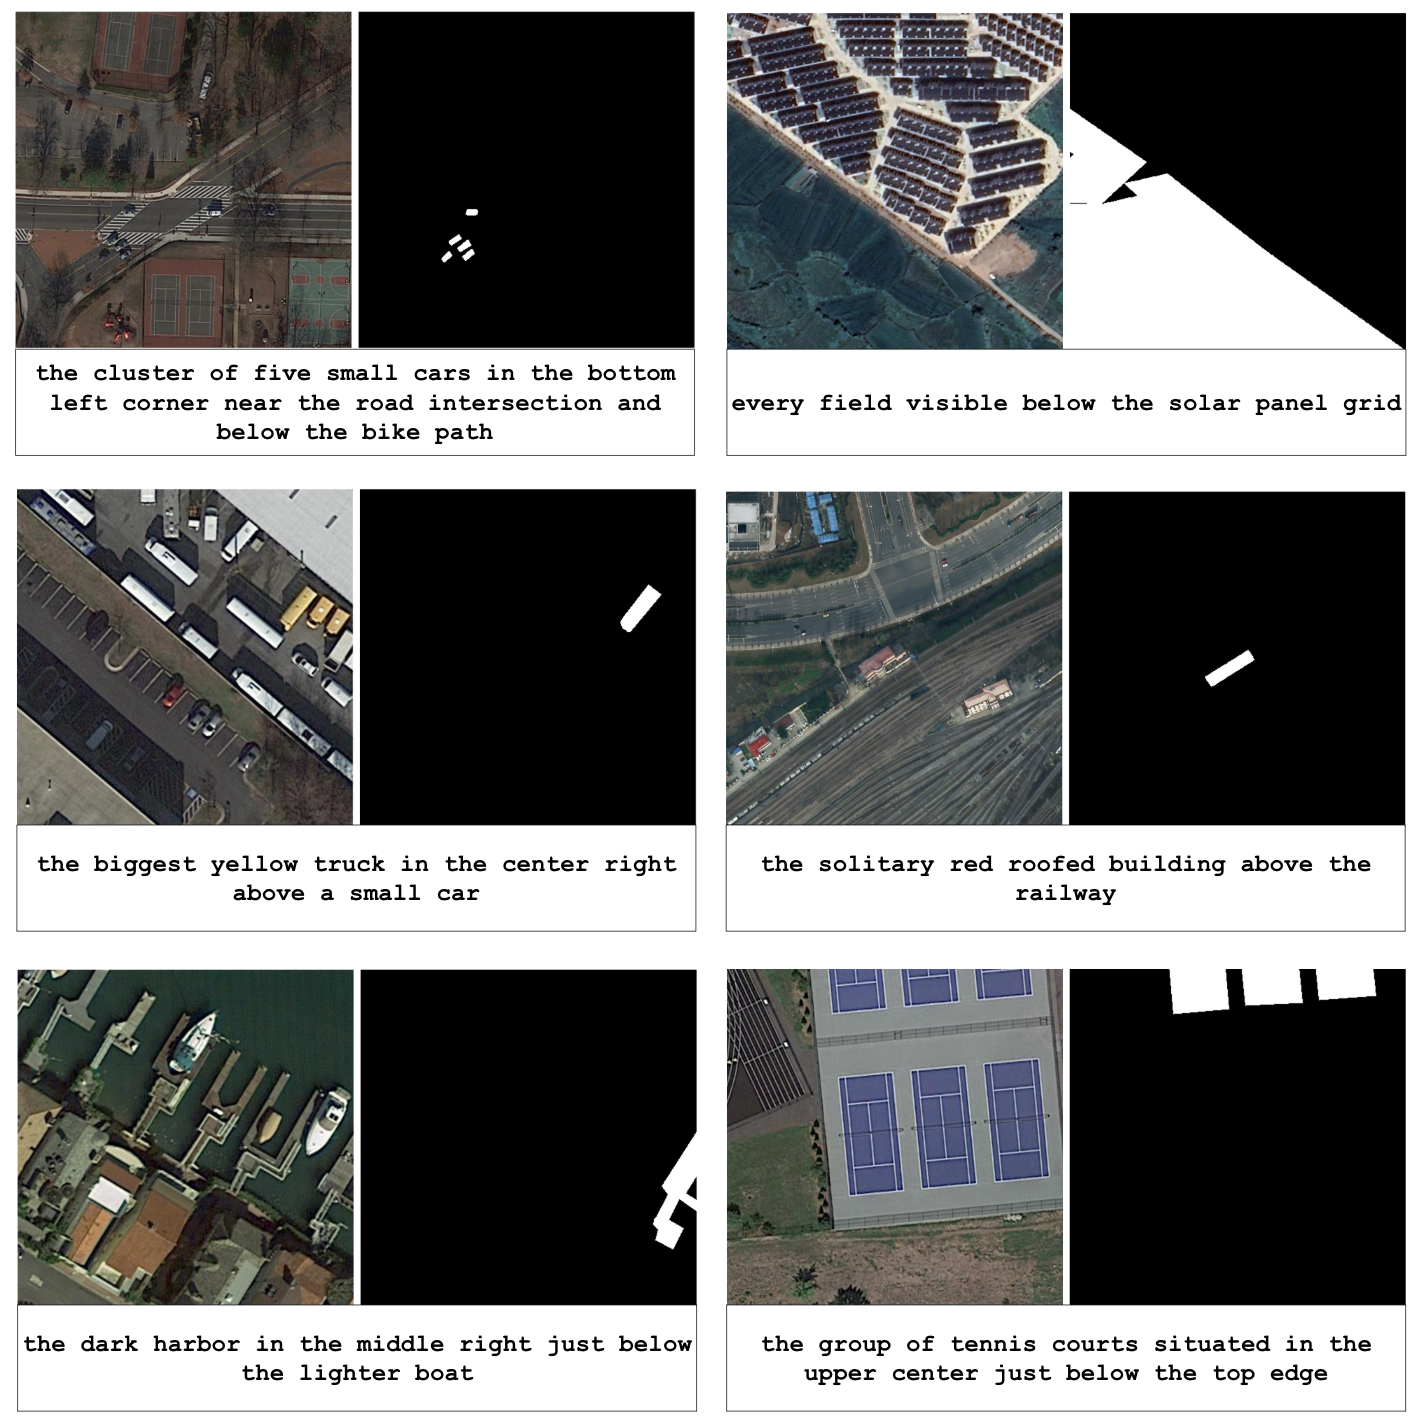
\includegraphics[width=\columnwidth]{./images/6samples.png}
\caption{Representative examples from Aerial-D dataset showing diverse referring expressions with corresponding aerial images and ground truth masks.}
\label{fig:dataset_examples}
\end{figure}
\endgroup


The key contributions of this work include: (1) a comprehensive toolchain that enables the production of complex referring expression datasets from instance/semantic segmentation datasets, including a rule-based pipeline, Large Language Model enhancement and distillation methods, and historic image data augmentation with dedicated filtering; (2) the construction of Aerial-D, a dataset comprising over 1.5 million expressions across 37,288 aerial image patches, created entirely through the proposed automatic pipeline; and (3) a unified model trained on Aerial-D alongside four additional datasets, leveraging historic transformations and other applicable components of the toolchain across the training data to deliver referring expression segmentation over instances, groups, classes, and land-cover regions while maintaining reliable performance on degraded historic imagery typical of archival aerial surveys.

\section{Related Work}
\label{sec:related}

This section reviews the datasets and architectural developments that underpin aerial image understanding, with emphasis on instance and semantic segmentation resources, referring expression segmentation datasets, historical imagery, and architectures tailored to remote sensing.

\subsection{Aerial Imagery Datasets}

Reliable progress in aerial image understanding depends on datasets that capture both discrete objects (e.g., ships, vehicles) and continuous land-cover (e.g., roads, water, vegetation), as well as datasets that test language-based selection of specific targets. This section first summarizes instance and semantic segmentation resources that established pixel-level ground truth, and then discusses the emergence of referring expression segmentation datasets that couple images, masks, and natural language.

\subsubsection{Instance and Semantic Segmentation}

The iSAID dataset~\cite{zamir2019isaid} established the foundation for instance segmentation in aerial imagery by providing 655,451 object instances across 15 categories in 2,806 high-resolution images. Building upon the DOTA dataset~\cite{xia2018dota}, iSAID addressed the unique challenges of aerial imagery including high object density, large scale variations, and arbitrary orientations. The dataset demonstrated that existing computer vision methods require specialized adaptation for aerial domains, as off-the-shelf approaches achieved suboptimal performance.

Complementing instance-level analysis, the LoveDA dataset~\cite{wang2021loveda} focused on land-cover semantic segmentation across urban and rural environments. Covering 536.15 km$^2$ with 0.3m resolution imagery, LoveDA enables domain adaptation research by addressing style differences between geographical environments, with urban scenes dominated by artificial objects and rural scenes containing natural elements.

\subsubsection{Referring Expression Segmentation Datasets}

While instance and semantic segmentation establish pixel-accurate supervision, they assume a fixed label set. Referring expression segmentation reframes the problem: given a natural language phrase, the goal is to select and segment the specific object (or group) described. In aerial imagery, this line of work began with RefSegRS~\cite{yuan2023rrsis}, which introduced 4,420 image--language--mask triplets and formalized Referring Remote Sensing Instance Segmentation (RRSIS). The dataset highlighted aerial-specific challenges—small, densely packed targets and cluttered layouts—where language can disambiguate between visually similar instances.

RRSIS-D~\cite{liu2024rotated} expanded both scale and annotation efficiency with 17,402 image--caption--mask triplets generated through a semi-automated pipeline using the Segment Anything Model (SAM)~\cite{sam}. The imagery originates from the DIOR dataset, grounding RRSIS-D in a broad remote-sensing corpus while leveraging automated mask generation. Beyond size, it targets aerial-specific phenomena—broad spatial scales and diverse object orientations—across 20 categories and seven attribute dimensions, enabling richer evaluation of language-guided selection in overhead scenes.

NWPU-Refer~\cite{yang2024large} further broadens coverage with 15,003 high-resolution images and 49,745 annotated targets spanning more than 30 countries. In contrast to semi-automated pipelines, it emphasizes purely manual annotation quality and explicitly supports single-object, multi-object, and non-object scenarios across 32 categories. Together, these datasets trace a steady shift from fixed-category segmentation toward language-conditioned, fine-grained selection in aerial imagery.

\subsubsection{Historical Imagery Applications}

Analysing historical aerial photographs introduces practical complications—reduced contrast, grayscale capture, film artifacts, and geometric distortions—yet these datasets are vital for studying long-term urban change. Urban1960SatSeg~\cite{hao2025urban1960satseg} addresses this gap with professionally annotated semantic segmentation over 1,240 km$^2$ of declassified mid-20th-century imagery from Xi'an, China. By focusing on degraded visual conditions, it provides a reference point for methods that must remain robust when applied to archival aerial data.

\subsection{Architectures for RRSIS}

Architectures for referring expression segmentation in aerial imagery combine vision backbones, language encoders, and fusion mechanisms that translate textual cues into pixel-level masks. The Rotated Multi-Scale Interaction Network (RMSIN)~\cite{liu2024rotated} is a representative design that builds bespoke processing blocks on top of a Swin Transformer~\cite{swin} visual encoder and a BERT~\cite{bert} language backbone. Its Intra-scale Interaction module refines fine-grained details with transformer~\cite{transformer} blocks, the Cross-scale Interaction module aligns multi-resolution features through cross-attention, and the Adaptive Rotated Convolution module injects rotation-aware convolutional filters to handle arbitrary object orientations.

MRSNet~\cite{yang2024large} adopts the same Swin~\cite{swin}--BERT~\cite{bert} backbone pairing but alters how features interact. Instead of RMSIN's triplet of modules, it employs hierarchical fusion that first consolidates information within each scale before exchanging context across scales, leading to a more progressive flow of visual detail toward the mask decoder. The shift in interaction pattern highlights how architectural variants largely differ in their feature fusion strategies rather than wholesale backbone changes.

RSRefSeg~\cite{chen2025rsrefseg} illustrates the alternative of leaning fully on large vision--language models. It replaces bespoke encoders with CLIP~\cite{clip} or SigLIP~\cite{siglip} for multimodal feature extraction and integrates SAM as the segmentation decoder. A lightweight AttnPrompter module converts language-conditioned features into sparse and dense prompts for SAM, while LoRA adapters fine-tune both CLIP/SigLIP and the SAM vision encoder to aerial imagery. Figure~\ref{fig:rsrefseg_arch} visualizes this configuration and highlights how the prompts interface with SAM. This design achieves the strongest reported IoU on RRSIS-D~\cite{liu2024rotated,chen2025rsrefseg} while requiring updates only to the bridging layers and low-rank adapters.
\begin{figure*}[t]
\centering
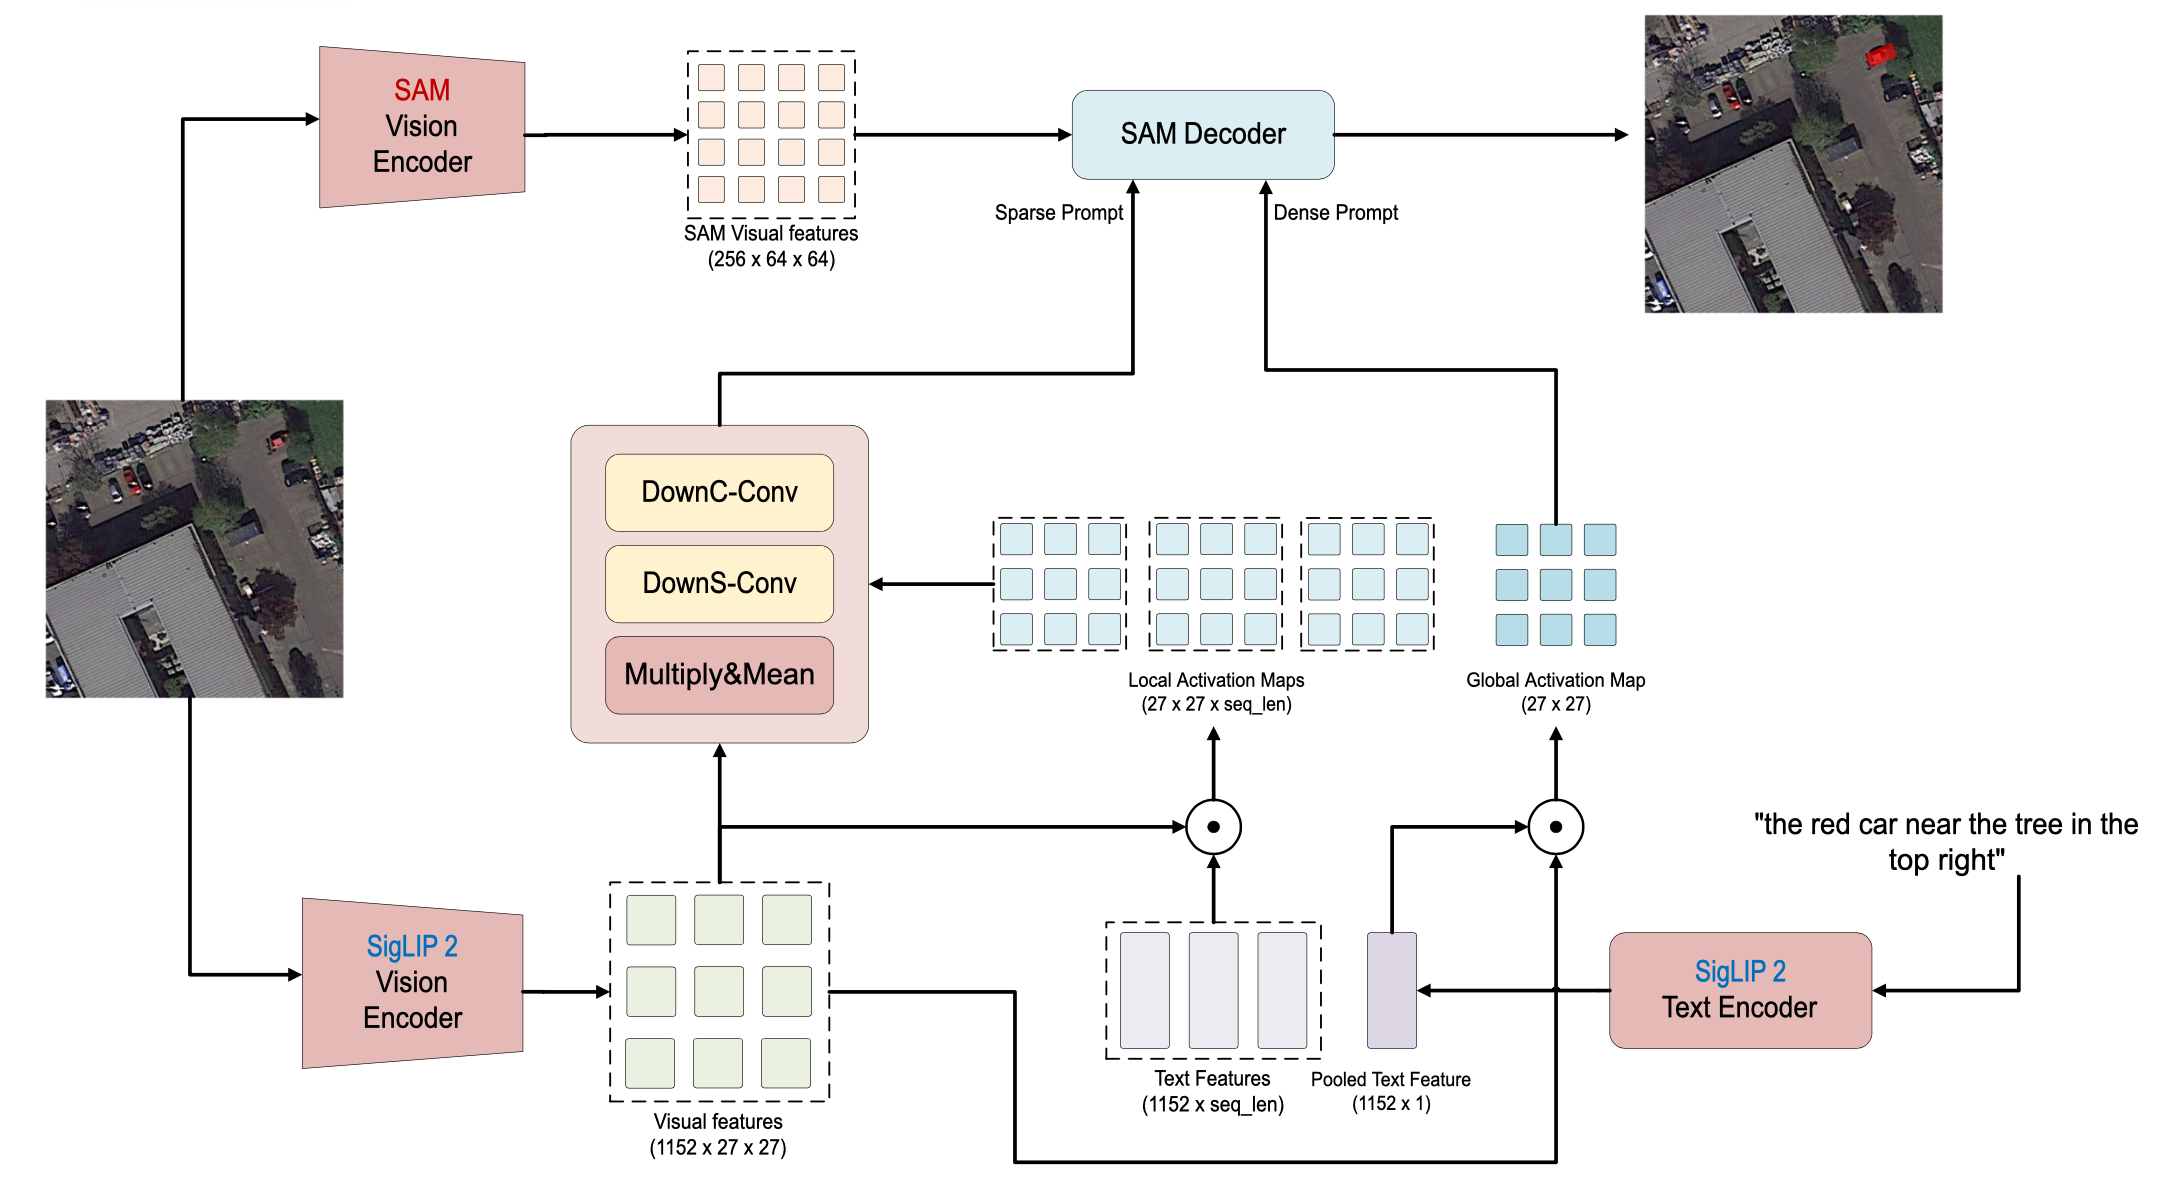
\includegraphics[width=0.9\textwidth]{./images/rsrefseg.png}
\caption{Overview of the RSRefSeg architecture~\cite{chen2025rsrefseg}, which couples a vision--language encoder with a segmentation decoder via a learned prompting bridge.}
\label{fig:rsrefseg_arch}
\end{figure*}

\subsection{Overview}

The current landscape of aerial image segmentation is shaped by three pillars that enable language-guided segmentation. First, instance and semantic datasets such as iSAID and LoveDA supply pixel-accurate supervision for objects and land-cover. Second, referring expression segmentation datasets including RefSegRS, RRSIS-D, and NWPU-Refer pair images with natural expressions and masks, enabling evaluation of language-conditioned target selection at varying scales and annotation regimes. Third, architectural developments span specialized remote-sensing networks (e.g., RMSIN, MRSNet) and foundation-model designs (e.g., RSRefSeg~\cite{chen2025rsrefseg}) that leverage strong vision and language backbones.

Crucially, the complementary supervision in iSAID and LoveDA presents an opportunity to construct a larger and more diverse referring expression segmentation resource by converting instance- and land-cover annotations into language-conditioned targets—motivating the creation of Aerial-D as a comprehensive dataset for aerial referring expressions.

Within this context, RSRefSeg stands out as a particularly compelling choice for referring expression segmentation: it benefits from powerful pretrained vision--language encoders (e.g., CLIP/SigLIP) and a high-capacity segmentation decoder (SAM) connected by a lightweight bridging mechanism. The resulting system establishes the leading IoU on RRSIS-D~\cite{chen2025rsrefseg}, demonstrating that foundation-model backbones can be adapted effectively to aerial referring expression segmentation.

\section{Aerial-D Dataset Construction}
\label{sec:approach}

This section details our comprehensive approach to constructing Aerial-D, a large-scale referring expression segmentation dataset for aerial imagery. Our methodology combines automated rule-based expression generation with a multimodal LLM expression component that is preceded by a cost-efficient distillation step, enabling both scale and linguistic diversity. We begin by establishing our source datasets, then describe our rule-based pipeline for generating referring expressions from existing annotations, followed by our distilled large language model enhancement procedure, and conclude with comprehensive dataset statistics demonstrating the scope and characteristics of the final resource.

\subsection{Source Datasets}

The Aerial-D dataset is constructed from two complementary aerial datasets with different annotation styles: iSAID (instance segmentation) and LoveDA (semantic segmentation). Together, these source datasets provide 21 distinct object and land-cover classes, with iSAID contributing 15 instance categories (e.g., vehicles, ships, buildings) and LoveDA contributing 6 semantic land-cover classes (e.g., farmland, forest, water).

We start by putting both sources into the same format so that a single model can learn from them side by side: square patches at $480\times480$. This size keeps small iSAID objects large enough to describe and segment, while fitting the input expectations of common vision encoders used in our model (e.g., CLIP/SigLIP image towers and SAM backbones\cite{clip,siglip,sam}).

We first resize the $1024\times1024$ LoveDA tiles directly to $480\times480$ while preserving their semantic masks. iSAID has uniquely high-resolution imagery with varying aspect ratios, so we instead slide a $480\times480$ window with overlap across each source image and keep the patches that contain valid instances. After these resizing steps, we run connected-component analysis on LoveDA to turn buildings and water into pseudo-instance targets—these categories tend to appear as isolated structures or bounded water bodies, making them natural candidates for instance-level descriptions. The remaining land-cover classes (e.g., farmland or forest) behave as contiguous surfaces, so we keep them as semantic regions and describe them holistically ("all agricultural land in the image"). The resulting per-patch representation retains instance targets, grouped semantic regions, and the original semantic labels that feed into the subsequent rule-guided expression generation.

\subsection{Rule-Based Expression Generation}

The core challenge is figuring out how to describe these target objects using only what we know from their bounding boxes, masks, and categories. We utilize the bounding box coordinates to understand where each object sits within the image patch. As shown in Figure \ref{fig:rule_example}, we divide each patch into a three-by-three grid marked with dotted lines, so we can say an object is "in the top right" or "in the center". When we have multiple objects of the same type, we also check if any are in extreme positions like the topmost or leftmost instance of that category.

Since we also have the pixel masks for each object, we can analyze their colors by looking at hue--saturation--value (HSV) distributions to distinguish between light and dark objects and a controlled palette of chromatic colors. We require at least 70\% dominance for achromatic labels ("light" or "dark") and a single hue to occupy at least 60\% of the chromatic pixels before we commit to a specific color; When neither threshold is met, no color descriptor is assigned and the cue is discarded. This thresholds ambiguous multi-hue regions and helps us ignore noisy signals that would otherwise mislead the language generation. We also avoid using color descriptors for buildings and water since these typically show mixed colors that aren't useful for identification.

We also create relationships between nearby objects by calculating angles between their positions, allowing us to generate expressions like "the ship to the left of the harbor" or "the vehicle above the building". The system uses eight directional relationships: above, below, to the left of, to the right of, and the four diagonal directions.

All these rules combine to generate various referring expressions for each object, as demonstrated in Figure \ref{fig:rule_example} where a single plane generates multiple possible descriptions including "the plane in the top right", "the light plane in the top right", and versions with relational descriptions. However, a significant challenge emerges when multiple objects end up with identical characteristics and generate the exact same expressions, creating ambiguous references where one phrase could describe multiple different objects. We solve this fundamental problem by taking the set of all expressions for all objects and targets in each image, matching them against each other to find duplicates, and when we find expressions that are identical, we cancel both expressions out and discard them as ambiguous. This filtering stage is crucial: it removes targets that cannot be uniquely verbalized using the rules alone, ensures the rule-based component only passes forward unambiguous instances, and guarantees that the downstream dataset never asks models to resolve intentionally ambiguous descriptions.

\begin{figure*}[t]
\centering
\begin{minipage}{0.5\textwidth}
\centering
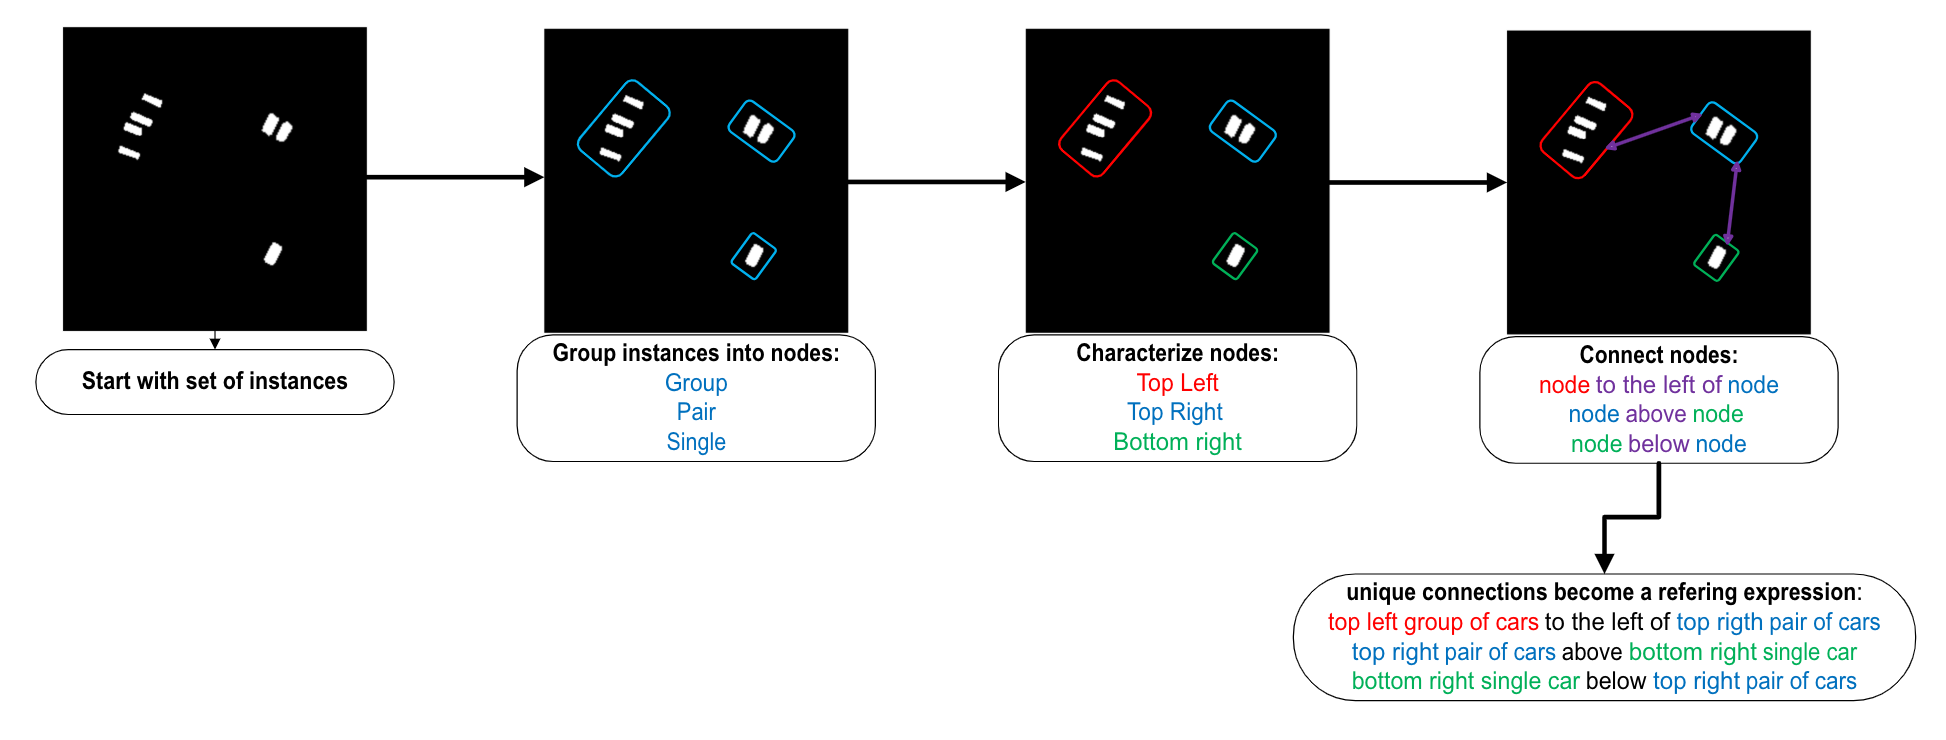
\includegraphics[width=0.65\textwidth]{./images/rule_based_generation.png}
\end{minipage}%
\begin{minipage}{0.5\textwidth}
\centering
\hspace{-1cm}
\raisebox{-0.3\height}{%
\resizebox{\textwidth}{!}{%
\footnotesize
\begin{tabular}{@{}ll@{}}
\toprule
\textbf{Rule Type} & \textbf{Example Instance} \\
\midrule
Category & "plane" \\
Grid Position & "in the top right" \\
Extreme Position & None \\
Color Classification & "light" \\
Directional Relations & "to the bottom right of a plane" \\
& "to the top right of a plane" \\
\midrule
\multicolumn{2}{l}{\textbf{Final Expressions}} \\
\multicolumn{2}{l}{"the plane in the top right"} \\
\multicolumn{2}{l}{"the light plane in the top right"} \\
\multicolumn{2}{l}{"the plane in the top right to the bottom right of a plane"} \\
\multicolumn{2}{l}{"the light plane in the top right to the bottom right of a plane"} \\
\multicolumn{2}{l}{"the plane in the top right to the top right of a plane"} \\
\multicolumn{2}{l}{"the light plane in the top right to the top right of a plane"} \\
\bottomrule
\end{tabular}%
}%
}

\end{minipage}
\caption{Example of rule generation for a single instance. The highlighted plane in the top right section demonstrates how the system assigns spatial, visual, and relational rules that will later be combined into referring expressions.}
\label{fig:rule_example}
\end{figure*}

\subsection{LLM Expression Generation}
\label{subsec:llm_expression_generation}
While rule-based expression generation provides a solid foundation for referring expression data, these expressions suffer from significant limitations in language variation and visual detail coverage. The rule-based approach produces linguistically constrained expressions with limited wording variations and lacks the ability to reference contextual elements beyond predefined source dataset categories.

To address these limitations, we employ a multimodal Large Language Model (LLM) to enhance our dataset by providing both images and expressions as input, enabling the model to rewrite and improve the original referring expressions. We prompt the LLM with two complementary tasks, as shown in Figure \ref{fig:llm_enhancement_example}. The first task focuses on linguistic variation, creating natural language alternatives for each rule-based expression without heavy reliance on visual cues. The second task uses visual information, where the model examines surrounding features in the image around the target object.

We overlap the target region with red bounding boxes to guide the model during the first task and pair each prompt with a focused close-up crop so that small or dense targets stay visible. For land-cover categories that lack crisp bounding boxes, we supply a dual-image prompt consisting of a masked overlay and the clean image, which helps the model anchor the relevant region. This combination of bounding box overlays, dual images, and mask prompts keeps the enhancement grounded on the correct area of the scene.

This dual-task prompting transforms basic expressions like "the group of 4 large vehicles in the top center" into linguistically diverse alternatives such as "the cluster of four big vehicles near the upper middle" and visually detailed descriptions like "the four large vehicles lined up side by side just below the pale paved strip at the very top middle", as shown in Figure~\ref{fig:llm_enhancement_example}. The model identifies and references contextual elements not captured in the original datasets, such as the "pale paved strip" and the "grassy area".

However, the full dataset contains approximately 300,000 captured targets including both objects and groups. To generate expressions, we process each target individually, meaning we would need 300,000 separate LLM requests. Using production-grade LLMs at this scale—for example, OpenAI’s o3 model\cite{o3} with strong visual capabilities—would cost thousands of dollars; Table \ref{tab:cost_comparison} reports the exact breakdown, making direct application prohibitively expensive for research-scale dataset construction.

To address this scalability challenge, we employ a knowledge distillation~\cite{hinton2015distilling} approach, as illustrated in Figure \ref{fig:llm_distillation}. We utilize OpenAI’s o3 model\cite{o3} and compare it against a much more lightweight open-weights model, Gemma3\cite{gemma3}. We obtain 500 high-quality outputs from o3 on a representative random subset of targets from the initial dataset. These outputs serve as training data for supervised fine-tuning using the parameter-efficient QLoRA method\cite{qlora} on Gemma3-12B.

During fine-tuning we apply LoRA adapters across both the text decoder and the SigLIP-derived vision stack embedded in Gemma3, which improves instruction adherence, suppresses hallucinations, and stabilizes the two-task output schema. The custom-tailored Gemma3 variant can then process all 300,000 targets on a single GPU while honoring the dual-task prompt structure—behavior the base Gemma3 model fails to follow reliably without distillation. Notably, the distilled model’s output quality approaches o3’s once fine-tuned; qualitative comparisons in Figure \ref{fig:distillation_comparison} show closely matched enhancements with markedly reduced hallucinations relative to the base Gemma3 model.

\begin{figure*}[t]
\centering
\begin{minipage}{0.5\textwidth}
\centering
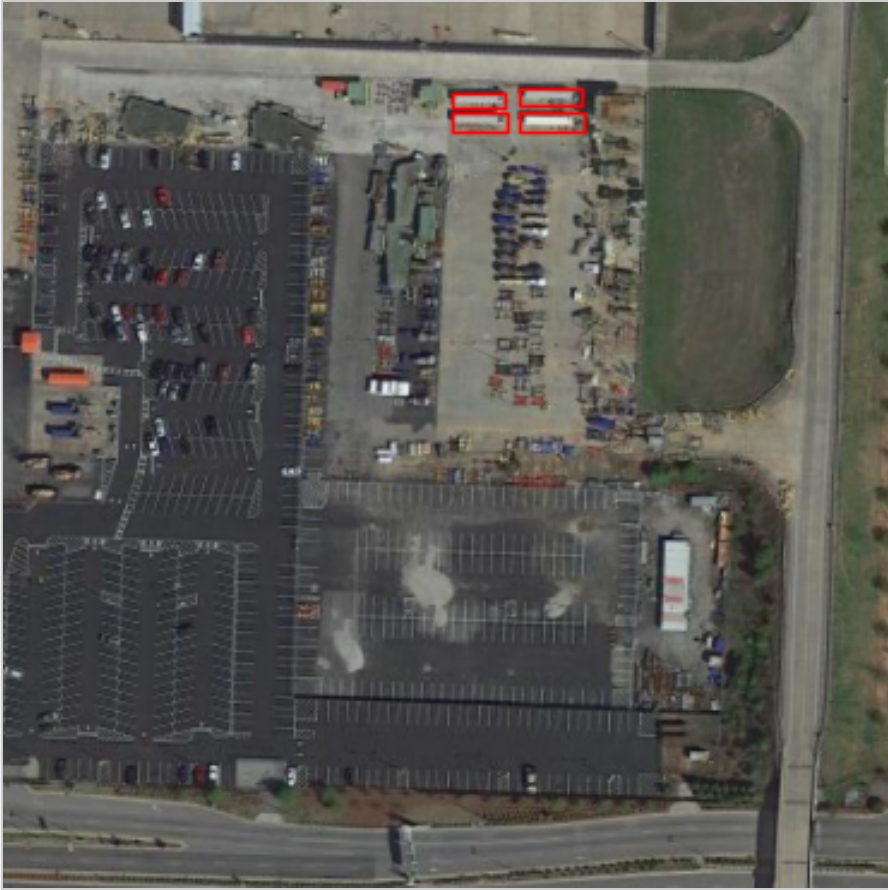
\includegraphics[width=0.65\textwidth]{./images/example_group.png}
\end{minipage}%
\begin{minipage}{0.5\textwidth}
\centering
\hspace{-1cm}
\raisebox{-0.3\height}{%
\footnotesize
\begin{tabular}{@{}p{2cm}p{5cm}@{}}
\toprule
\textbf{Expression Type} & \textbf{Example} \\
\midrule
Original & the group of 4 large vehicles in the top center \\
\midrule
Enhanced & the cluster of four big vehicles near the upper middle \\
\midrule
Unique & the four large vehicles lined up side by side just below the pale paved strip at the very top middle \\
\midrule
Unique & the set of four big vehicles parked in a single row in the upper center beside the grassy area to the right \\
\bottomrule
\end{tabular}%
}
\end{minipage}
\caption{Example of LLM enhancement process showing original aerial image with group of four large vehicles (left) and corresponding expression enhancements (right).}
\label{fig:llm_enhancement_example}
\end{figure*}

\subsection{Historic Image Filter Augmentation}
\label{subsec:historic_filters}

In order to improve robustness to archival image conditions, we augment training with three parametric transformations that reproduce characteristic degradations of historical aerial photographs (Figure~\ref{fig:historic_filters}). These filters are applied on the fly during training rather than baked into the dataset, so each mini-batch can include either a clean or a historically degraded view of the same patch.

Let $I_{orig}(x)\in[0,255]^3$ denote the RGB image at pixel $x$, and let $\operatorname{clip}(\cdot)$ clamp values to $[0,255]$.

We simulate grayscale capture by converting to luminance, as in \eqnref{eq:gray}:
\begin{equation}
I_{\text{bw}}(x) = 0.299\,R(x) + 0.587\,G(x) + 0.114\,B(x).
\label{eq:gray}
\end{equation}

To emulate film response and grain, we first apply a mild gamma adjustment (\eqnref{eq:gamma}), then a linear contrast change around the mean (\eqnref{eq:contrast}), followed by additive Gaussian noise (\eqnref{eq:grain}):
\begin{equation}
I_{\gamma}(x) = 255\,\big(I_{\text{bw}}(x)/255\big)^{\gamma}.
\label{eq:gamma}
\end{equation}
\begin{equation}
I_{c}(x) = \big(I_{\gamma}(x) - \mu\big)\,c + \mu.
\label{eq:contrast}
\end{equation}
\begin{equation}
I_{\text{grain}}(x) = \operatorname{clip}\big(I_{c}(x) + \eta(x)\big),\quad \eta(x)\sim\mathcal{N}(0,\sigma^2).
\label{eq:grain}
\end{equation}
We use $\gamma=1.2$, $c=0.8$, and $\sigma=0.1\times 255$ to produce mild contrast loss and film grain.

Finally, we apply a fixed sepia transform (\eqnref{eq:sepia}) followed by uniform sensor/scan noise (\eqnref{eq:sepia_noise}):
\begin{equation}
\begin{bmatrix} S_R(x) \\ S_G(x) \\ S_B(x) \end{bmatrix}
= \operatorname{clip}\left(
\begin{bmatrix}
0.272 & 0.534 & 0.131 \\
0.349 & 0.686 & 0.168 \\
0.393 & 0.769 & 0.189
\end{bmatrix}
\begin{bmatrix} R(x) \\ G(x) \\ B(x) \end{bmatrix}
\right).
\label{eq:sepia}
\end{equation}
\begin{equation}
I_{\text{sepia}}(x) = \operatorname{clip}\big(\mathbf{S}(x) + \xi(x)\big),\quad \xi(x)\sim\mathcal{U}(0,50).
\label{eq:sepia_noise}
\end{equation}

These effects mimic tonal range reduction, lens grain, and scanning artifacts typical of mid-century aerial photography while preserving the spatial structure that segmentation relies on. Figure~\ref{fig:historic_filters} illustrates the visual impact of each transformation.

\begin{figure*}[t]
\centering
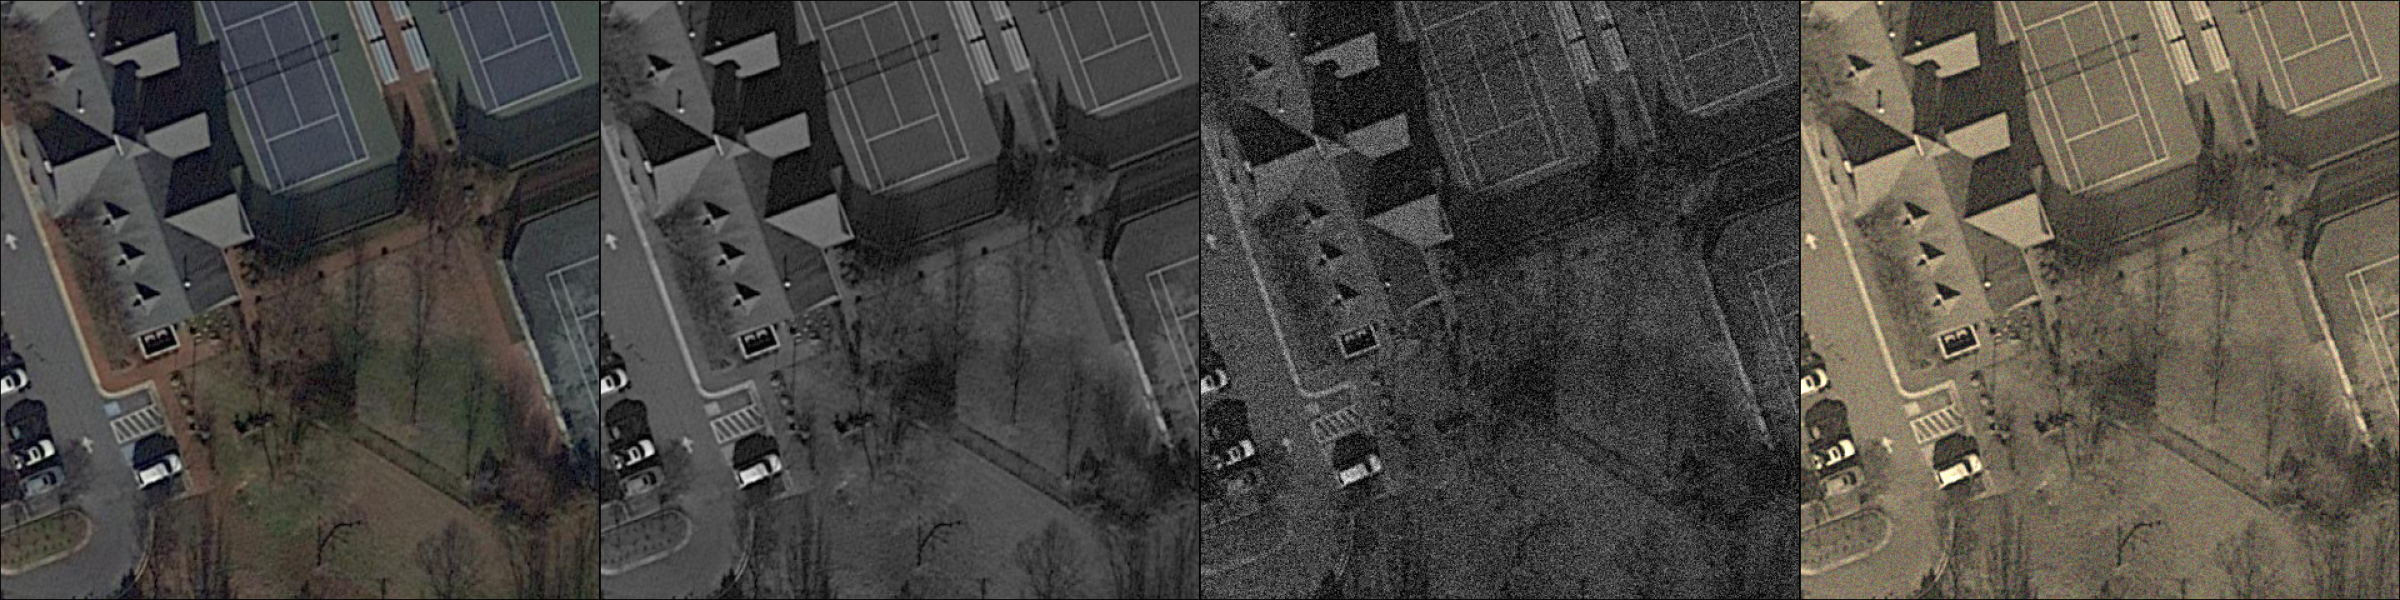
\includegraphics[width=0.9\textwidth]{./images/filters.png}
\caption{Comparison of original aerial image patch with three historic filter transformations: grayscale conversion, sepia toning, and Gaussian noise addition. These filters simulate common degradation patterns in historical aerial photography.}
\label{fig:historic_filters}
\end{figure*}

\subsection{Final Dataset Statistics}

The rule-based generation yields 506,194 starting expressions and identifies 259,709 annotated targets across the corpus (Table~\ref{tab:llm_enhancement_stats}). Building on this base, the LLM enhancement is prompted to produce one language variation for each original expression and two unique visual-detail expressions for each target, adding 496,895 and 519,434 expressions respectively and resulting in 1,522,523 total expressions. Of these, 1,278,453 expressions describe discrete instances or groups, while 244,070 cover the land-cover regions that remain at the semantic level. Figure~\ref{fig:expression_wordcloud} illustrates how this process expands the vocabulary.

\begin{figure}[!t]
\centering
\includegraphics[width=\columnwidth]{./images/expression_wordcloud.png}
\caption{Word cloud visualization of the most frequent terms in Aerial-D referring expressions, highlighting the domain-specific vocabulary and spatial descriptors characteristic of aerial imagery.}
\label{fig:expression_wordcloud}
\end{figure}

\begin{figure*}[t]
\centering
\begin{minipage}{0.48\textwidth}
\centering
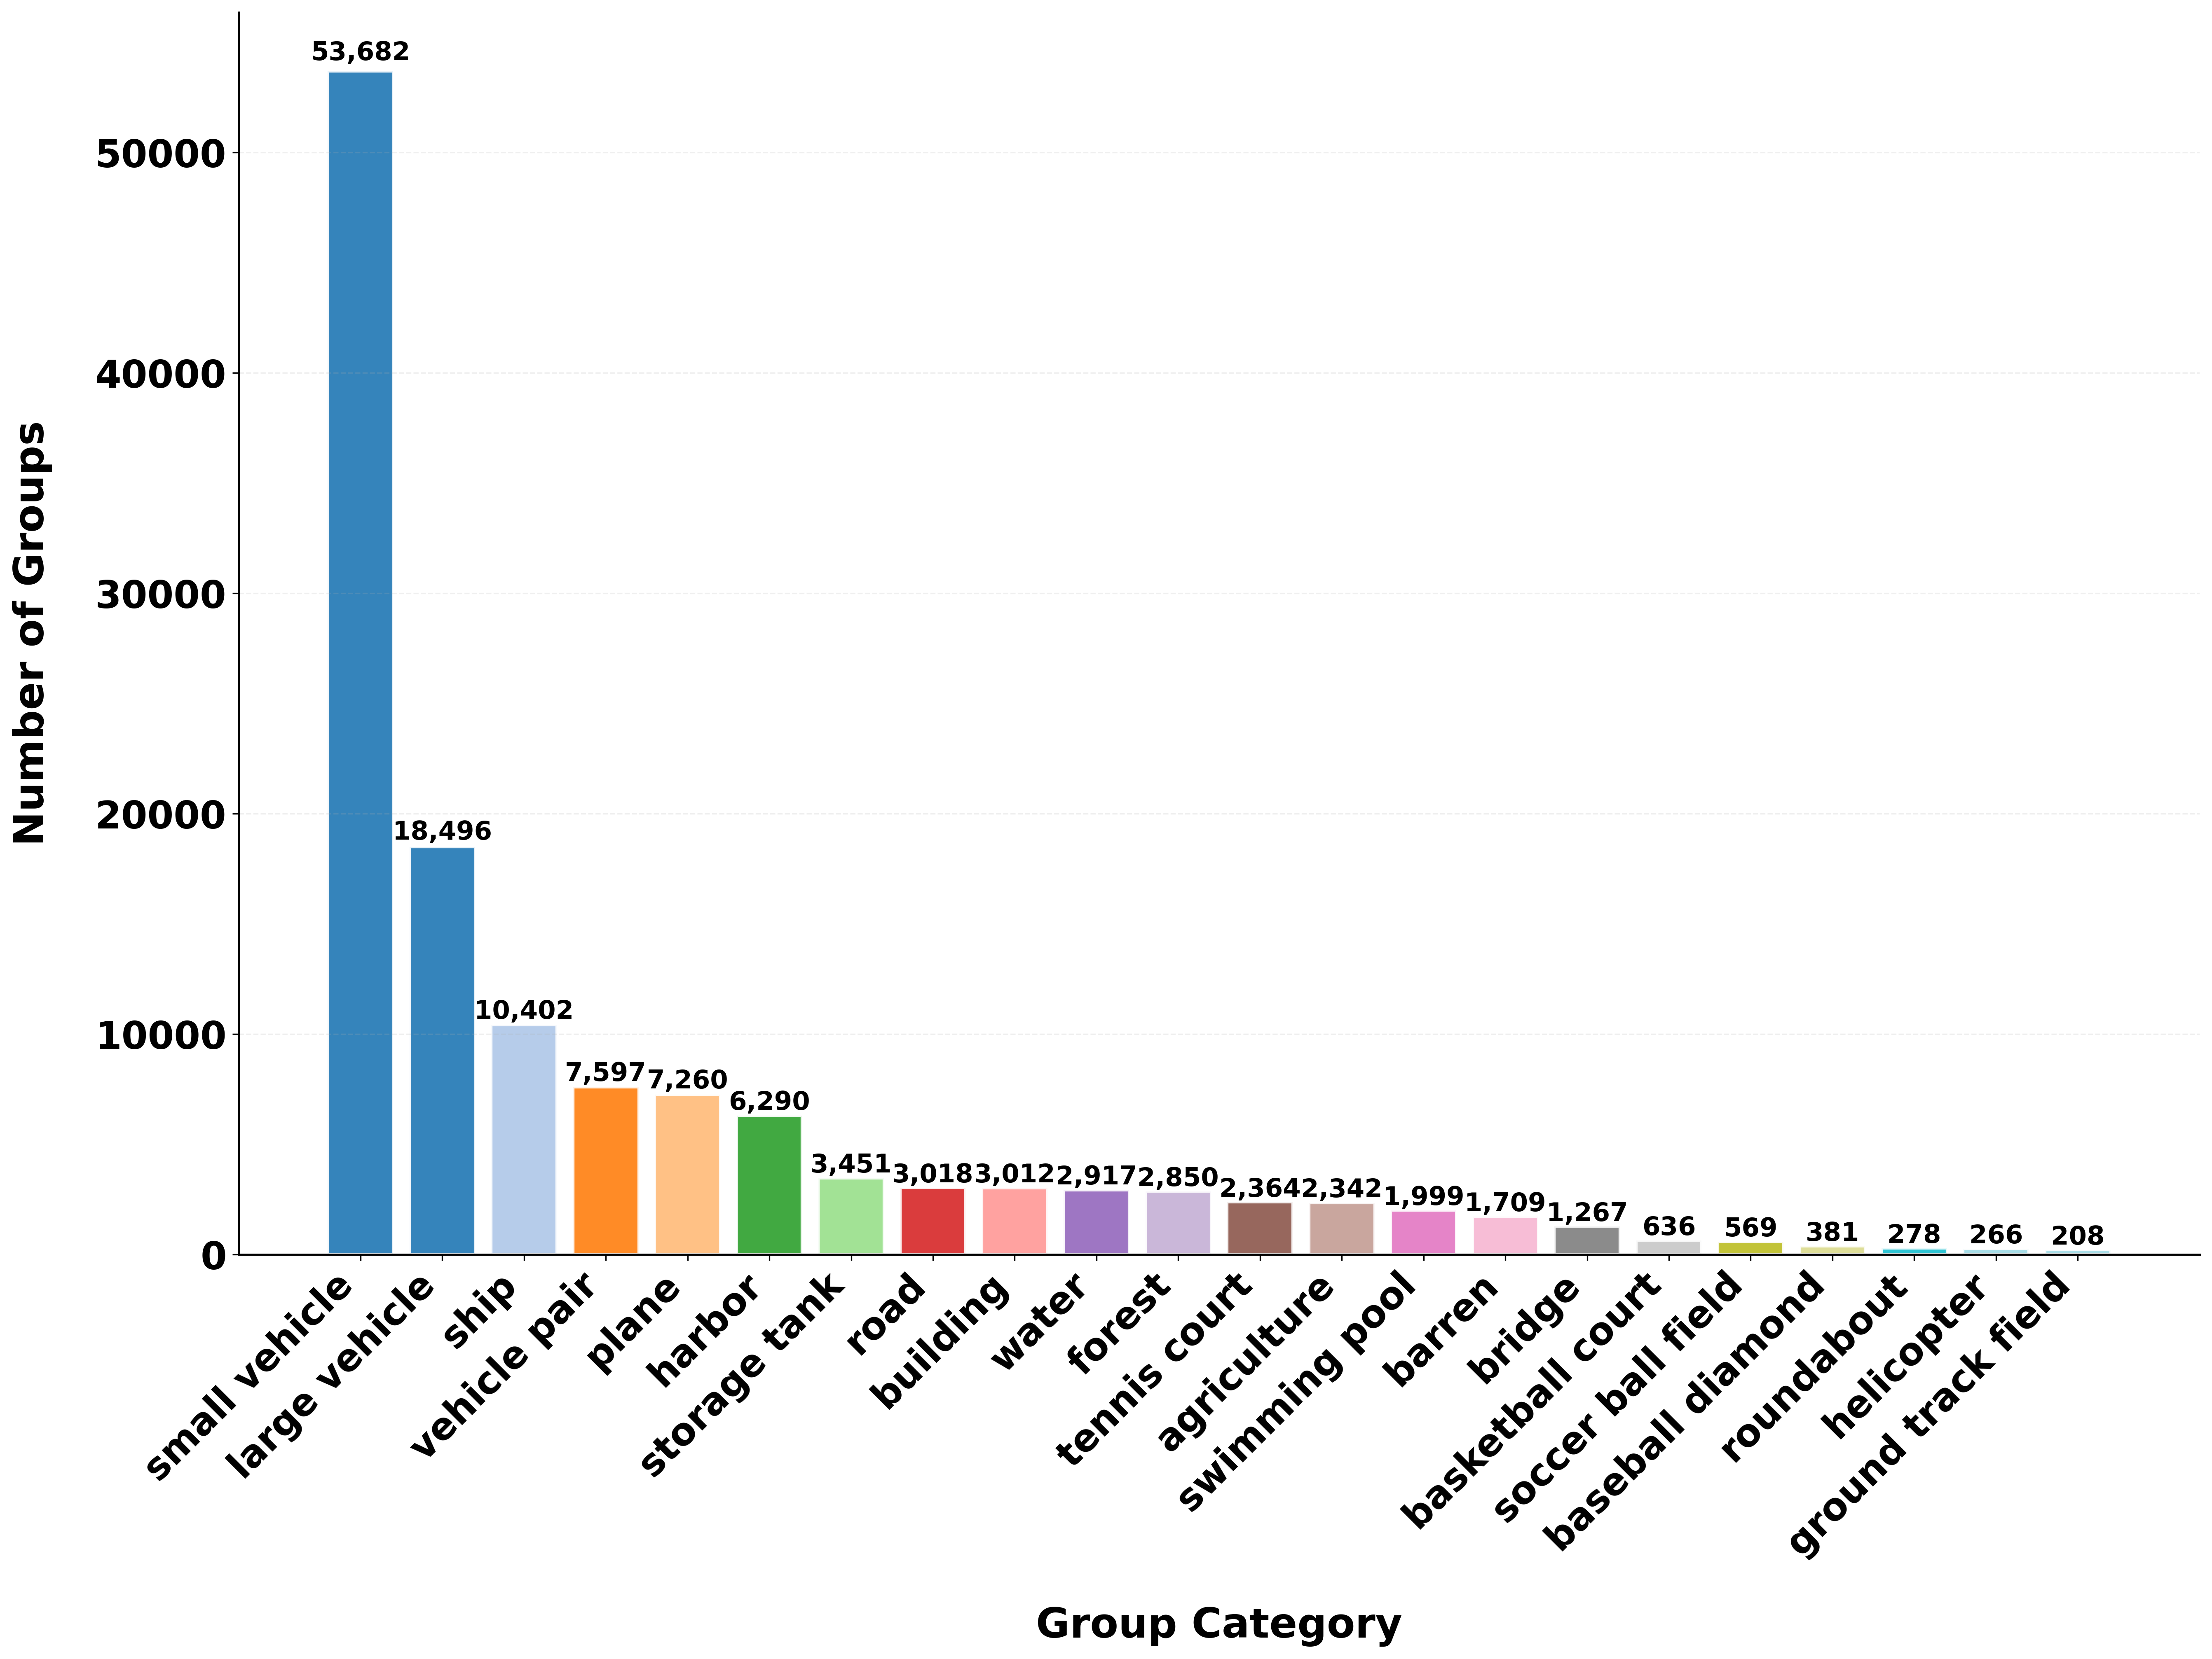
\includegraphics[width=\textwidth]{./images/group_category_distribution.png}
\end{minipage}\hfill
\begin{minipage}{0.48\textwidth}
\centering
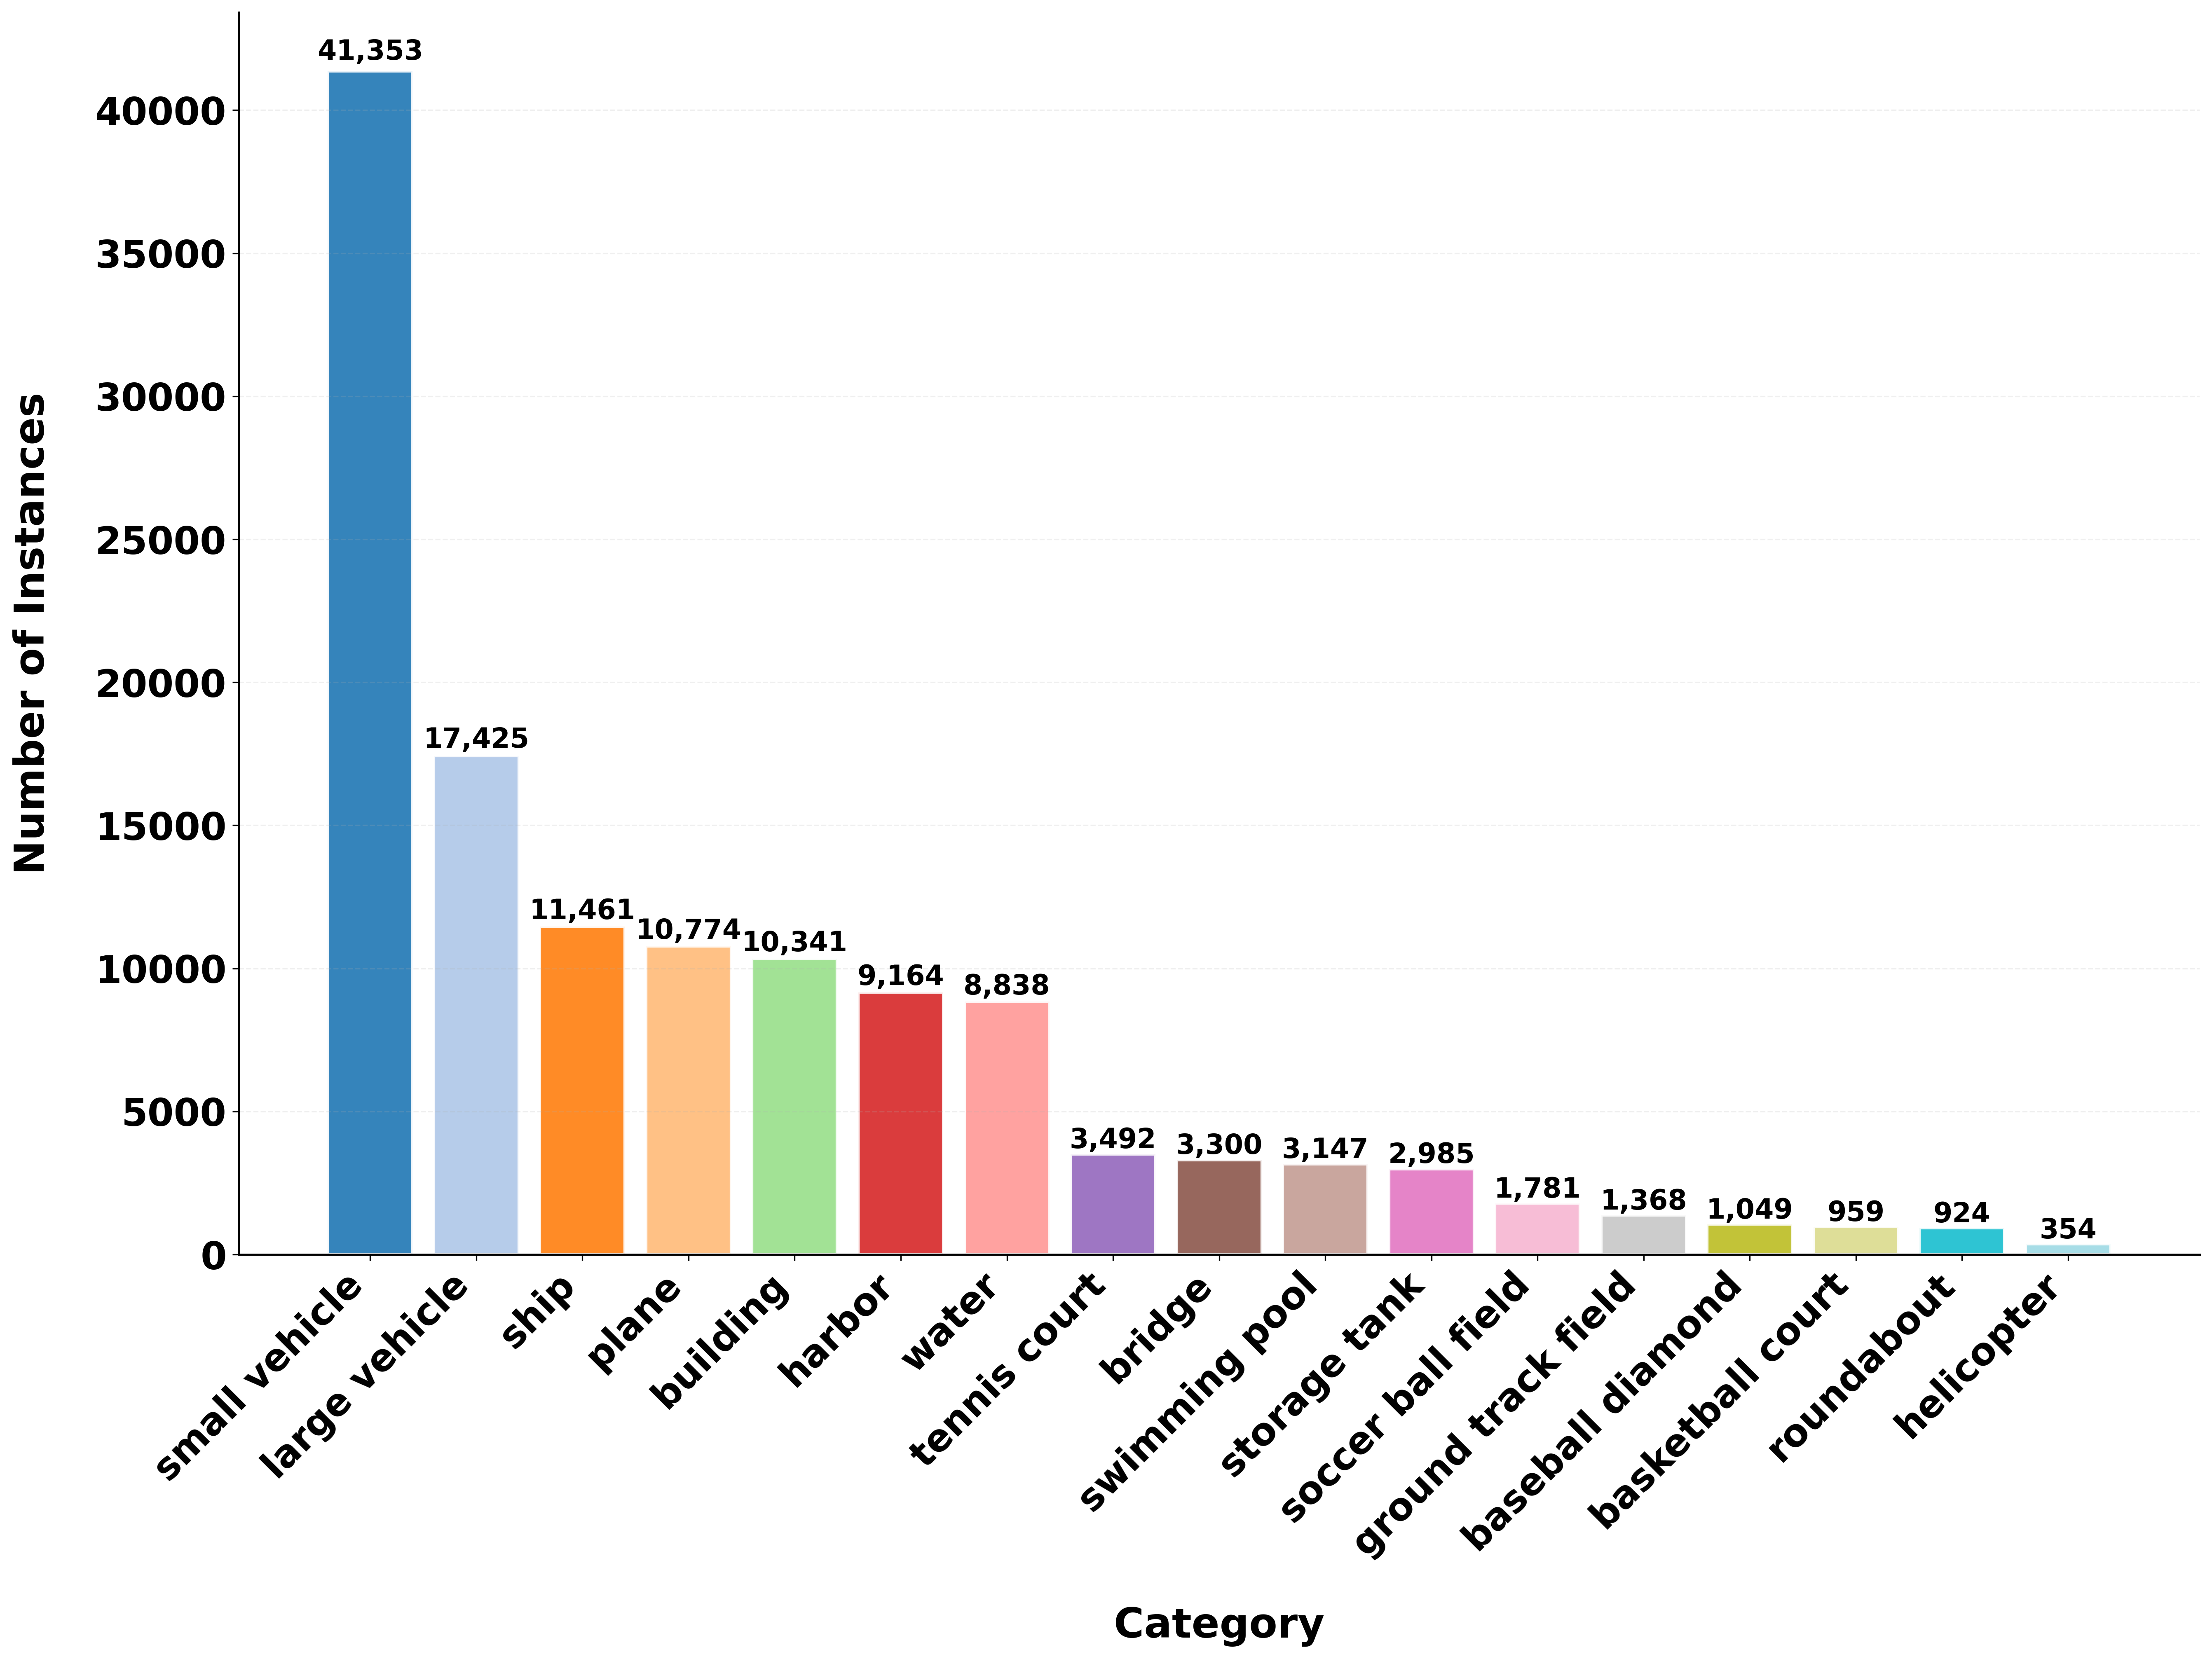
\includegraphics[width=\textwidth]{./images/instance_category_distribution.png}
\end{minipage}
\caption{Category distribution analysis of the Aerial-D dataset. Left: Distribution of grouped and semantic targets showing the prevalence of region-level categories in the corpus. Right: Distribution of individual instance annotations across semantic categories, demonstrating the dataset's coverage of aerial object types.}
\label{fig:category_distributions}
\end{figure*}

Table~\ref{tab:dataset_comparison} compares Aerial-D with prior RRSIS datasets and shows how it scales along three axes: images, targets per image, and expressions per target. First, Aerial-D contains nearly three times as many images as previous datasets. Second, each image typically includes many segmented targets. Third, each target is paired with multiple referring expressions. The table also clarifies how the corpus splits between the 1.28 million instance-level expressions and the 244 thousand semantic expressions that describe the land-cover categories, a combination that is absent from earlier datasets. Together, these factors yield more than 1.5 million referring expressions, positioning Aerial-D among the largest publicly available RRSIS resources. Beyond scale, Aerial-D relies on a fully automatic pipeline that combines rule-based generation with LLM enhancement, supports both single-object and multi-object references, and preserves the original category balance as illustrated in Figure~\ref{fig:category_distributions}.

\begin{table*}[t]
\centering
\caption{Comparison with Existing RRSIS Datasets}
\label{tab:dataset_comparison}
\resizebox{\textwidth}{!}{%
\begin{tabular}{@{}lcccccccc@{}}
\toprule
\textbf{Dataset} & \textbf{Image Resolution} & \textbf{Images} & \textbf{Instance Expr.} & \textbf{Semantic Expr.} & \textbf{Single-object} & \textbf{Multi-object} & \textbf{Patch Size} & \textbf{Annotation Generation} \\
\midrule
RefSegRS & 0.13m & 4,420 & 4,420 & -- & \checkmark & $\times$ & 512 & Manual \\
RRSIS-D & 0.5m--30m & 17,402 & 17,402 & -- & \checkmark & $\times$ & 800 & Semi-auto \\
NWPU-Refer & 0.12m--0.5m & 15,003 & 49,745 & -- & \checkmark & \checkmark & 1,024--2,048 & Manual \\
\midrule
\multirow{2}{*}{\textbf{Aerial-D}} & \multirow{2}{*}{\textbf{0.3m--4.5m}} & \multirow{2}{*}{\textbf{37,288}} & \textbf{1,278,453} & -- & \textbf{\checkmark} & \textbf{\checkmark} & \multirow{2}{*}{\textbf{480}} & \multirow{2}{*}{\textbf{Automated + LLM}} \\
 & & & -- & \textbf{244,070} & $\times$ & \textbf{\checkmark} & & \\
\bottomrule
\end{tabular}%
}
\end{table*}

\begin{table}[t]
\centering
\caption{Expression Distribution by Source}
\label{tab:llm_enhancement_stats}
\footnotesize
\begin{tabular}{@{}lccc@{}}
\toprule
\textbf{Source} & \textbf{Train} & \textbf{Validation} & \textbf{Total} \\
\midrule
Rule-Based & 371K & 135K & 506K \\
LLM Language Variations & 364K & 133K & 497K \\
LLM Visual Variations & 382K & 137K & 519K \\
\midrule
\textbf{Total} & \textbf{1,118K} & \textbf{405K} & \textbf{1,523K} \\
\bottomrule
\end{tabular}
\end{table}

\begin{figure}[!b]
\centering
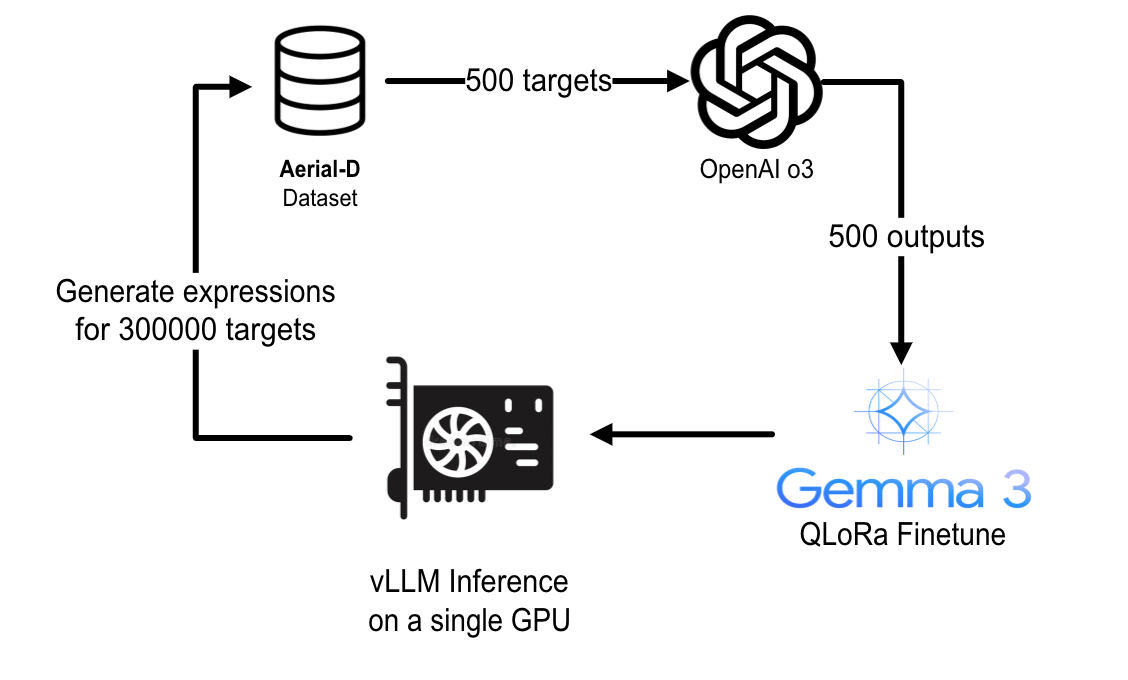
\includegraphics[width=\columnwidth]{./images/distillation.png}
\caption{Knowledge distillation pipeline for scalable LLM enhancement. A small sample of 500 expressions is processed through OpenAI's o3 model\cite{o3} to generate high-quality training targets, which are then used to fine-tune Gemma3-12B\cite{gemma3} via QLoRA\cite{qlora}. The fine-tuned model enables cost-effective local inference to enhance the full dataset using vLLM\cite{vllm} on a single GPU.}
\label{fig:llm_distillation}
\end{figure}

\section{Experiments}
\label{sec:experiments}

This section presents a comprehensive experimental evaluation of Aerial-D that spans model training, cross-dataset generalization, and targeted ablations. We begin by outlining the RSRefSeg backbone and training configuration, then report cross-dataset results on established aerial referring expression segmentation datasets. Beyond aggregate performance, we also include: (i) ablation of expression enhancement strategies; (ii) ablation of historic-filter training; and (iii) qualitative comparison across language models (o3, base Gemma3, and our distilled Gemma3-Aerial model), coupled with a cost analysis of these alternatives.

\subsection{Model Architecture}
\label{subsec:model_architecture}

Evaluating Aerial-D demands a model that preserves the link between natural-language instructions and precise masks while handling densely packed aerial targets. RSRefSeg meets these requirements and already demonstrated state-of-the-art results on RRSIS-D\cite{liu2024rotated}. We reimplemented the architecture in PyTorch~\cite{pytorch} and verified those RRSIS-D gains before extending the system to Aerial-D, which confirmed that the design transfers reliably to new datasets.

Our reimplementation of RSRefSeg\cite{chen2025rsrefseg} mirrors the original component pairing: SigLIP2\cite{siglip2} supplies the image--text encoder and SAM\cite{sam} provides the mask decoder. We fine-tune both modules with Low-Rank Adaptation (LoRA)\cite{lora} layers placed on the query and value projections of each Vision Transformer\cite{vit} encoder block and on the query, key, value, and output projections of the text encoder. Two checkpoints appear throughout the experiments. RSRefSeg-b keeps SAM-ViT-Base and LoRA rank $r=16$ for a lighter configuration, whereas RSRefSeg-l upgrades to SAM-ViT-Large with rank $r=32$ to maximize capacity while preserving the same training recipe.

\subsection{Experimental Setup}
\label{subsec:experimental_setup}

Training adheres to the RSRefSeg recipe so that differences arise from the data rather than from custom optimization. Batches contain four samples with gradient accumulation of two steps, yielding an effective batch size of eight. All experiments run on a single NVIDIA RTX~A6000 GPU. Both RSRefSeg-b and RSRefSeg-l follow the same training recipe, with RSRefSeg-b using SAM-ViT-Base and LoRA rank $r=16$ for a lighter configuration, while RSRefSeg-l uses SAM-ViT-Large with rank $r=32$ to maximize capacity. The combined model uses \texttt{SigLIP2-SO400M} for language--vision encoding at $384\times384$ resolution and \texttt{SAM-ViT-Large} at $1024\times1024$ for mask decoding, with LoRA rank $r=32$ steering the adaptation. We employ AdamW\cite{adamw} with learning rate $1\times10^{-4}$, weight decay 0.01, polynomial decay (power 0.9), mixed precision\cite{mixedprecision}, and gradient clipping at 1.0 to mirror the original training dynamics. During the data preparation phase of training, we apply one of the three historic filters (selected with equal probability) to 20\% of training images in each non-historic dataset. Note that Urban1960SatSeg is inherently historic imagery, so it receives no additional filtering and provides direct supervision for archival conditions.

In order to keep the cross-dataset mix balanced, Aerial-D contributes only the \emph{LLM Visual Variations} subset highlighted in Section~\ref{subsec:ablation_studies}. That ablation shows this subset carries the strongest signal while still covering every target; limiting Aerial-D to these expressions keeps the millions of available sentences from overwhelming the four public datasets, each of which supplies only tens of thousands of annotations. The combined run therefore spans Aerial-D (LLM Visual Variations), RRSIS-D\cite{liu2024rotated}, NWPU-Refer\cite{yang2024large}, RefSegRS\cite{yuan2023rrsis}, and Urban1960SatSeg\cite{hao2025urban1960satseg}. Validation follows the official splits, and Aerial-D relies on the full validation split (405K expressions), which is further broken down into instance targets and semantic regions in Table~\ref{tab:aeriald_variants}. To probe robustness we also evaluate fully filtered validation sets for Aerial-D, RRSIS-D, NWPU-Refer, and RefSegRS by converting every image with one of the three historic filters. Scores for those variants appear in the "Hist." columns.

\subsection{Evaluation Results}
\label{subsec:evaluation_results}

Tables~\ref{tab:aeriald_variants} and \ref{tab:combined_training_results} report validation results for the combined model trained jointly on all datasets. Both tables focus on mean IoU~\cite{everingham2010pascal} and overall IoU for the original validation splits alongside their historic-filtered counterparts, highlighting aggregate overlap rather than thresholded pass rates.

Table~\ref{tab:aeriald_variants} isolates Aerial-D and reports validation performance by target type. Instance targets correspond to explicit objects or groups, while the "All Targets" column aggregates both instance- and semantic-level references across the full 405K validation expressions. These values serve as baseline checkpoints for future work that evaluates new architectures on Aerial-D.

Across the external datasets in Table~\ref{tab:combined_training_results}, the RSRefSeg-b and RSRefSeg-l checkpoints remain competitive with previously published results despite being trained within a single unified pipeline. That schedule blends five datasets, applies historic filters to more than 20\% of the training imagery, and supervises both instance- and semantic-level targets drawn from Aerial-D. Historic columns illustrate that the LoRA-tuned RSRefSeg-l retains accuracy under simulated degradations, closing the gap between clean and historic imagery without requiring dataset-specific adjustments. The same table also foregrounds how the larger checkpoint strengthens overall IoU on RefSegRS and NWPU-Refer while maintaining the strong RRSIS-D performance reported in prior work.

The performance gap on RefSegRS deserves particular attention: while RMSIN achieves 59.96\% mIoU, RSRefSeg-l reaches 44.52\%. This gap reflects distribution shift, as RefSegRS contains referring patterns (e.g., vehicles along specific roads) that differ significantly from Aerial-D, RRSIS-D, and NWPU-Refer. Multi-dataset training biases the model toward the majority distribution, causing lower performance on out-of-distribution RefSegRS samples.

The combined evaluation therefore remains competitive with published references across every dataset while providing reproducible Aerial-D baselines. The modest gap between the original and historic evaluations confirms that injecting filtered imagery during training delivers robustness without eroding accuracy on contemporary photographs.

\begin{table*}[t]
\centering
\caption{Aerial-D supervision variants evaluated on the validation split (historic scores in \textcolor{blue}{blue}).}
\label{tab:aeriald_variants}
\resizebox{\textwidth}{!}{%
\begin{tabular}{@{}l|cc|cc|cc@{}}
\toprule
\multirow{2}{*}{\textbf{Model}} & \multicolumn{2}{c|}{\textbf{Instance Targets}} & \multicolumn{2}{c|}{\textbf{Semantic Targets}} & \multicolumn{2}{c}{\textbf{All Targets}} \\
\cmidrule(lr){2-3} \cmidrule(lr){4-5} \cmidrule(lr){6-7}
 & \textbf{mIoU} & \textbf{oIoU} & \textbf{mIoU} & \textbf{oIoU} & \textbf{mIoU} & \textbf{oIoU} \\
\midrule
\textbf{RSRefSeg-b (ours)} & 49.78\% / \textcolor{blue}{46.82\%} & 63.44\% / \textcolor{blue}{61.12\%} & 47.21\% / \textcolor{blue}{43.08\%} & 61.50\% / \textcolor{blue}{58.73\%} & 49.12\% / \textcolor{blue}{45.92\%} & 62.98\% / \textcolor{blue}{60.58\%} \\
\textbf{RSRefSeg-l (ours)} & 52.94\% / \textcolor{blue}{49.10\%} & 66.07\% / \textcolor{blue}{63.02\%} & 50.83\% / \textcolor{blue}{46.74\%} & 64.82\% / \textcolor{blue}{61.15\%} & 52.50\% / \textcolor{blue}{48.50\%} & 65.80\% / \textcolor{blue}{62.80\%} \\
\bottomrule
\end{tabular}%
}
\end{table*}

\begin{table*}[t]
\centering
\caption{Cross-dataset validation results for RSRefSeg variants (ours) and published baselines (historic scores in \textcolor{blue}{blue}; "--" indicates metrics not reported in the cited work).}
\label{tab:combined_training_results}
\resizebox{\textwidth}{!}{%
\begin{tabular}{@{}l|cc|cc|cc|cc@{}}
\toprule
\multirow{2}{*}{\textbf{Model}} & \multicolumn{2}{c|}{\textbf{RefSegRS}} & \multicolumn{2}{c|}{\textbf{RRSIS-D}} & \multicolumn{2}{c|}{\textbf{NWPU-Refer}} & \multicolumn{2}{c}{\textbf{Urban1960SatSeg}} \\
\cmidrule(lr){2-3} \cmidrule(lr){4-5} \cmidrule(lr){6-7} \cmidrule(lr){8-9}
 & \textbf{mIoU} & \textbf{oIoU} & \textbf{mIoU} & \textbf{oIoU} & \textbf{mIoU} & \textbf{oIoU} & \textbf{mIoU} & \textbf{oIoU} \\
\midrule
\textbf{RSRefSeg-b (ours)} & 24.81\% / \textcolor{blue}{17.54\%} & 40.89\% / \textcolor{blue}{29.41\%} & 64.37\% / \textcolor{blue}{61.16\%} & 76.83\% / \textcolor{blue}{75.44\%} & 39.42\% / \textcolor{blue}{33.15\%} & 59.52\% / \textcolor{blue}{\textbf{56.56\%}} & \textbf{70.65\%} & \textbf{88.86\%} \\
\textbf{RSRefSeg-l (ours)} & 44.52\% / \textcolor{blue}{\textbf{36.03\%}} & 55.74\% / \textcolor{blue}{\textbf{45.74\%}} & \textbf{65.37\%} / \textcolor{blue}{\textbf{62.61\%}} & 76.33\% / \textcolor{blue}{\textbf{76.03\%}} & \textbf{45.75\%} / \textcolor{blue}{\textbf{39.11\%}} & 62.75\% / \textcolor{blue}{55.29\%} & 69.74\% & 88.73\% \\
\midrule
RMSIN\cite{liu2024rotated,yang2024large,chen2025rsrefseg} & \textbf{59.96\%} & \textbf{76.81\%} & 62.27\% & 76.50\% & 41.75\% & 62.66\% & -- & -- \\
RSRefSeg-b\cite{chen2025rsrefseg} & -- & -- & 63.68\% & 76.05\% & -- & -- & -- & -- \\
RSRefSeg-l\cite{chen2025rsrefseg} & -- & -- & 64.67\% & \textbf{77.24\%} & -- & -- & -- & -- \\
MRSNet\cite{yang2024large} & -- & -- & -- & -- & 44.86\% & \textbf{63.59\%} & -- & -- \\
Urban1960SatUSM\cite{hao2025urban1960satseg} & -- & -- & -- & -- & -- & -- & 68.80\% & -- \\
\bottomrule
\end{tabular}%
}
\end{table*}

\subsection{LLM Expression Generation Ablation}
\label{subsec:ablation_studies}

To measure how synthetic language affects segmentation, we retrain RSRefSeg on Aerial-D while isolating the different expression sources. The goal is to contrast the original rule-generated sentences against those produced by the LLM pipeline and determine which variants provide the strongest supervision. We adopt the lighter RSRefSeg-b configuration—SAM-ViT-Base with LoRA rank $r=16$—so each run completes quickly while preserving the optimization settings from Section~\ref{subsec:experimental_setup}.

Using this setup, we train four separate models, each exposed to a distinct slice of Aerial-D: (i) \emph{Rule-based Only} retains the deterministic descriptions produced by the rule system; (ii) \emph{LLM Language Variations} relies on rewrites that diversify the wording while preserving the target; (iii) \emph{LLM Visual Variations} selects LLM augmentations that inject alternative visual cues; and (iv) \emph{Combined All} unites the three sources. Figure~\ref{fig:llm_enhancement_example} illustrates how the enhanced variants expand the phrasing beyond the rule-based baseline. We evaluate the resulting checkpoints on four validation sets without additional tuning: Aerial-D (using the 405K-expression validation split) and three external datasets—RefSegRS, RRSIS-D, and NWPU-Refer—to observe how each expression type supports generalization beyond the training distribution.

Table~\ref{tab:ablation_expression_types} summarizes the results and explicitly reports both the number of \emph{Samples} and \emph{Epochs} used per configuration. Looking across datasets, several consistent patterns emerge. On Aerial-D, the \emph{Combined All} configuration achieves the best accuracy, which is expected given that the validation distribution matches that training mixture. For the three external datasets, different subsets yield the strongest generalization: on RRSIS-D, the \emph{LLM Language Variations} run delivers the highest scores; on NWPU-Refer, emphasizing varied visual cues through \emph{LLM Visual Variations} is most beneficial; and on RefSegRS, uniting the three sources provides the best results. These outcomes highlight the breadth of ways to phrase referring expressions and show that leveraging LLMs to introduce targeted variety improves cross-dataset generalization.

In order to keep early stopping responsive to each subset, we monitor validation loss across the four runs and halt training as soon as it begins to rebound. Because the \emph{Combined All} subset is roughly three times larger than the others, its validation loss ticks upward immediately after the second epoch, so we stop that run at two epochs. The three smaller subsets continue improving through the fourth epoch before showing the same rise, allowing four full passes over their data. This schedule means that the language-variation and visual-variation models actually process fewer total samples than the combined run, yet they surpass it on RRSIS-D and NWPU-Refer. The outcome reveals that curated expression subsets can be more sample efficient than the full mixture, which is why the combined model in Section~\ref{subsec:evaluation_results} draws on the LLM Visual Variations split of Aerial-D. Beyond sample efficiency, constraining Aerial-D to that subset keeps the cross-dataset mix from being dominated by a single corpus whose expression pool would otherwise reach into the millions.

\begin{table*}[t]
\centering
\caption{Expression Enhancement Ablation Across Four Datasets}
\label{tab:ablation_expression_types}
\resizebox{\textwidth}{!}{%
\begin{tabular}{@{}lcc|cc|cc|cc|cc@{}}
\toprule
\multirow{2}{*}{\textbf{Training Configuration}} & \multirow{2}{*}{\textbf{Samples}} & \multirow{2}{*}{\textbf{Epochs}} & \multicolumn{2}{c|}{\textbf{Aerial-D}} & \multicolumn{2}{c|}{\textbf{RefSegRS}} & \multicolumn{2}{c|}{\textbf{RRSIS-D}} & \multicolumn{2}{c}{\textbf{NWPU-Refer}} \\
\cmidrule(lr){4-5} \cmidrule(lr){6-7} \cmidrule(lr){8-9} \cmidrule(lr){10-11}
 & & & \textbf{mIoU} & \textbf{oIoU} & \textbf{mIoU} & \textbf{oIoU} & \textbf{mIoU} & \textbf{oIoU} & \textbf{mIoU} & \textbf{oIoU} \\
\midrule
Rule-based Only & 371K & 4 & 34.57\% & 39.31\% & 3.73\% & 0.55\% & 34.22\% & 36.46\% & 16.78\% & 13.70\% \\
LLM Language Variations & 364K & 4 & 46.45\% & 56.99\% & 5.75\% & 4.99\% & \textbf{41.63\%} & \textbf{42.48\%} & 21.89\% & 16.68\% \\
LLM Visual Variations & 382K & 4 & 46.54\% & 63.02\% & 18.32\% & 8.37\% & 31.78\% & 33.73\% & \textbf{24.68\%} & \textbf{29.22\%} \\
Combined All & 1,118K & 2 & \textbf{49.33\%} & \textbf{64.30\%} & \textbf{18.80\%} & \textbf{8.58\%} & 34.07\% & 34.80\% & 24.57\% & 28.27\% \\
\bottomrule
\end{tabular}%
}
\end{table*}

\subsection{Distillation Ablation: Gemma3 vs. o3 Model Comparison}
\label{subsec:distillation_ablation}

This ablation measures how the generator choice inside the LLM enhancement stage affects expression quality and overall cost. We evaluate three options for producing the enhanced expressions: OpenAI’s o3, the off-the-shelf Gemma3-12B, and the distilled Gemma3-Aerial model described in Section~\ref{subsec:llm_expression_generation} (see Figure~\ref{fig:llm_distillation}).

All three models are prompted and decoded in the same way so that differences stem from the generator rather than the interface. The base Gemma3 baseline frequently ignores the dual-task schema, hallucinates objects that are not present, and references the guiding bounding boxes inside the expression, which undermines segmentation training. Distillation sharply reduces those errors, producing grounded descriptions that resemble the o3 outputs while remaining accessible on local hardware.

Table~\ref{tab:cost_comparison} quantifies the practical impact. Running o3 across $\sim$300,000 targets would cost roughly \$6.2K, whereas the distilled Gemma3 produces comparable guidance for about \$26—roughly $238\times$ cheaper because inference runs locally instead of via a commercial API. Figure~\ref{fig:distillation_comparison} illustrates why the student is worth training: the base Gemma3 hallucinates a second baseball diamond that does not exist, while the distilled variant stays aligned with the image and mirrors the grounded detail that o3 provides.

\begin{table}[t]
\centering
\caption{Cost Analysis: Gemma3 vs. o3 Model for Large-Scale Annotation (cost calculations based on API pricing with average request token counts)}
\label{tab:cost_comparison}
\resizebox{\columnwidth}{!}{%
\begin{tabular}{@{}lcc@{}}
\toprule
\textbf{Model} & \textbf{Cost per request} & \textbf{Cost for 300K requests} \\
\midrule
o3 Model & \$0.020728 & \$6,218.32 \\
Distilled Gemma3 & \$0.000087 & \$26.01 \\
\midrule
\textbf{Savings} & \textbf{$238\times$ cheaper} & \textbf{\$6,192.31 (99.6\%)} \\
\bottomrule
\end{tabular}%
}
\end{table}

\begin{figure*}[t]
\centering
\begin{minipage}{0.5\textwidth}
\centering
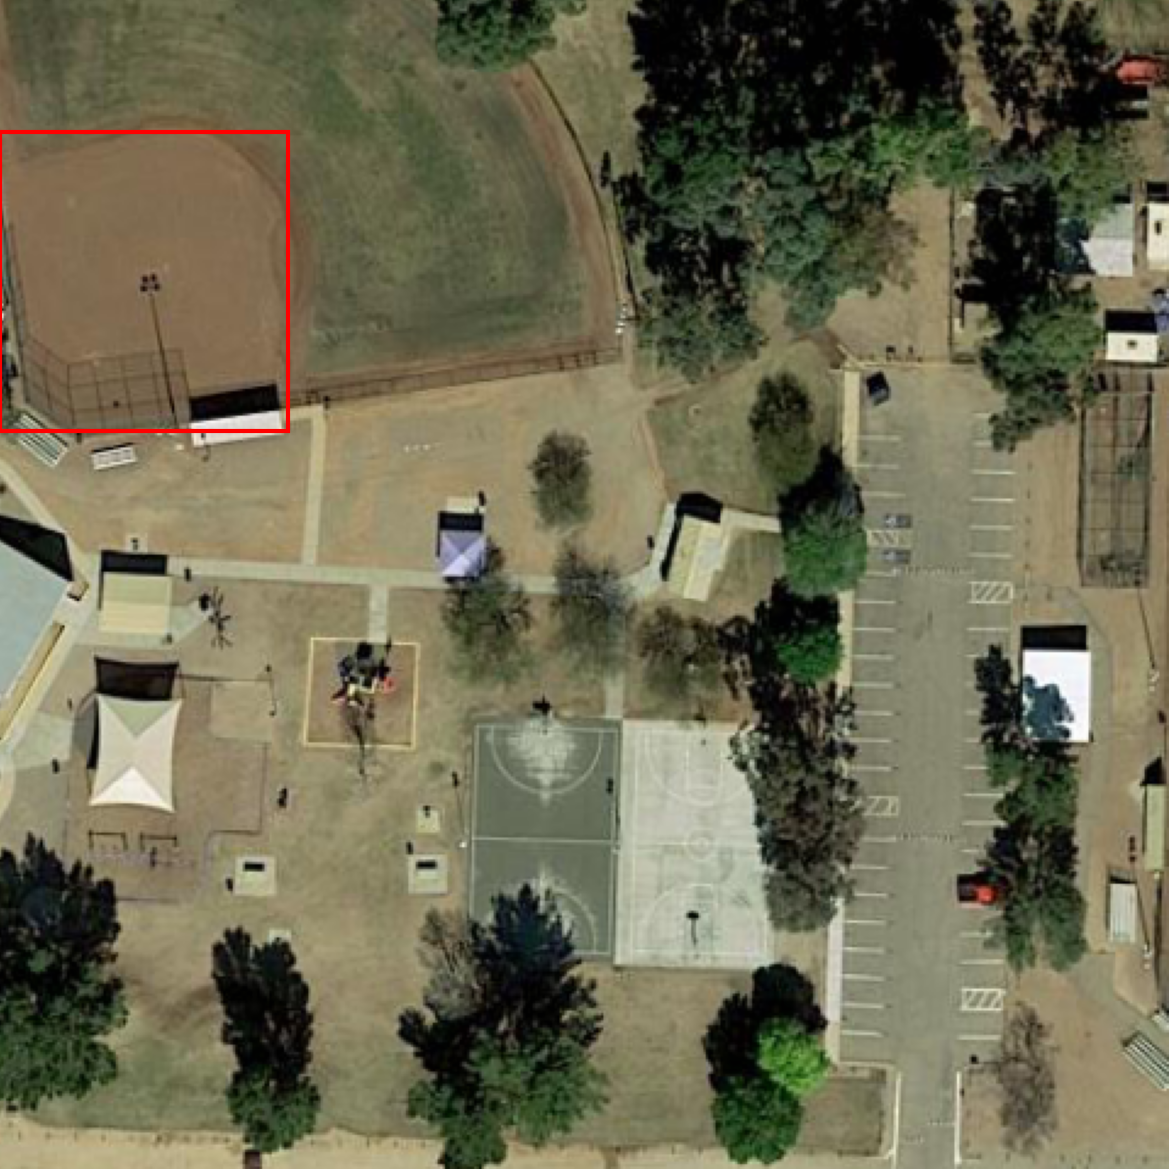
\includegraphics[width=0.65\textwidth]{./images/3llm.png}
\end{minipage}%
\begin{minipage}{0.5\textwidth}
\centering
\hspace{-1cm}
\raisebox{-0.3\height}{%
\footnotesize
\begin{tabular}{@{}p{2cm}p{5cm}@{}}
\toprule
\textbf{Expression Type} & \textbf{Example} \\
\midrule
Original & the orange baseball diamond in the top left \\
\midrule
o3 & the orange baseball diamond with the light pole near home plate in the upper left \\
\midrule
Gemma3 Base & the bright orange baseball diamond to the left of another similar baseball diamond in the top left \\
\midrule
Gemma3-Aerial-12B & the orange baseball field with a chainlink fence surrounded by grass to the north and trees to the west \\
\bottomrule
\end{tabular}%
}
\end{minipage}
\caption{Qualitative comparison between o3, the base Gemma3 model, and our fine-tuned Gemma3-Aerial-12B on the same aerial scene. Each model receives the identical rule-based prompt and decoding setup, revealing how their rewritten expressions differ under matched conditions.}
\label{fig:distillation_comparison}
\end{figure*}

\subsection{Historic Filter Ablation Study}
\label{subsec:historic_ablation}

In order to understand how much the historic-image filters described in Section~\ref{subsec:historic_filters} contribute to robustness, we repeat the combined training without injecting those filters. Models that only encounter clean, contemporary imagery typically falter when historic photographs suddenly introduce monochrome toning, contrast loss, or sepia casts. We therefore run an ablation that removes the filters from the training mix and compares the resulting model against the full recipe, using the RSRefSeg-b variant because its SAM-ViT-Base backbone trains faster and lets us report results alongside the base model in Table~\ref{tab:combined_training_results}.

Table~\ref{tab:historic_ablation_results} summarises both setups. Each row lists the clean mIoU (Orig.), the historic counterpart (Hist., in \textcolor{blue}{blue}), and the drop relative to the full-training baseline. Removing filters keeps the Orig. values aligned with Table~\ref{tab:combined_training_results} yet costs five to nine points on the historic splits. Excluding Urban1960SatSeg is far more damaging: the model recovers less on the filtered datasets, collapses to roughly 18\% mIoU on Urban1960SatSeg, and loses the only source of direct historic supervision. Synthetic filters therefore help, but real historic imagery remains necessary because Urban1960SatSeg introduces different land-cover labels—such as treating buildings as area classes—and includes considerably more noise than the other datasets.

\begin{table*}[t]
\centering
\caption{Historic-filter ablations. Each row lists the clean score followed by the historic-filter variant (blue) with percentage-point deltas relative to Table~\ref{tab:combined_training_results}; the second row also removes Urban1960SatSeg supervision.}
\label{tab:historic_ablation_results}
\renewcommand{\arraystretch}{1.1}
\resizebox{\textwidth}{!}{%
\begin{tabular}{@{}l|cc|cc|cc|c@{}}
\toprule
\multirow{2}{*}{\textbf{Training Setup}} & \multicolumn{2}{c|}{\textbf{RRSIS-D (mIoU)}} & \multicolumn{2}{c|}{\textbf{NWPU-Refer (mIoU)}} & \multicolumn{2}{c|}{\textbf{RefSegRS (mIoU)}} & \multicolumn{1}{c}{\textbf{Urban1960SatSeg (mIoU)}} \\
\cmidrule(lr){2-3} \cmidrule(lr){4-5} \cmidrule(lr){6-7}
 & \textbf{Orig.} & \textbf{Hist.} & \textbf{Orig.} & \textbf{Hist.} & \textbf{Orig.} & \textbf{Hist.} & \textbf{Orig.} \\
\midrule
No Filters & 64.30\% & \textcolor{blue}{55.00\%} (\textcolor{red}{-6.16}) & 39.50\% & \textcolor{blue}{27.50\%} (\textcolor{red}{-5.65}) & 24.80\% & \textcolor{blue}{12.00\%} (\textcolor{red}{-5.54}) & 69.00\% (\textcolor{red}{-1.65}) \\
No Filters + No Urban1960SatSeg & 63.00\% & \textcolor{blue}{56.00\%} (\textcolor{red}{-5.16}) & 38.00\% & \textcolor{blue}{29.00\%} (\textcolor{red}{-4.15}) & 23.50\% & \textcolor{blue}{13.50\%} (\textcolor{red}{-4.04}) & 18.00\% (\textcolor{red}{-52.65}) \\
\bottomrule
\end{tabular}%
}
\renewcommand{\arraystretch}{1}
\end{table*}

Values in parentheses denote percentage-point change relative to the baseline combined model in Table~\ref{tab:combined_training_results}; \textcolor{blue}{blue} marks historic-filtered validation scores.

\section{Conclusion and Future Work}
\label{sec:conclusion}

This work introduces Aerial-D together with an end-to-end methodology that converts existing aerial segmentation datasets into a large-scale repository of referring expressions. The pipeline begins with a rule-driven generator that translates masks into prose grounded on location, appearance, and relational cues, then refines that language through LLM rewriting while keeping costs manageable via a distilled Gemma3 annotator. The resulting corpus enables RSRefSeg to be trained jointly across five datasets, establishes reproducible baselines on Aerial-D, and remains competitive with published results on RRSIS-D, NWPU-Refer, RefSegRS, and Urban1960SatSeg. By pairing these evaluations with ablations on expression sources and historic-image filters, we demonstrate that Aerial-D delivers a harder dataset for referring segmentation in aerial photos and highlights the specific ingredients that improve robustness.

Future work can extend this foundation in three directions. First, the expression-enhancement pipeline can be applied directly to the native captions supplied with public datasets such as RRSIS-D and NWPU-Refer, enriching their language with the visual grounding cues that proved effective for Aerial-D and creating a unified, higher-variety training pool. Second, multilingual variants of these expressions can be produced while preserving full automation by pairing high-quality translation models with our distillation recipe—either prompting o3 and training a Gemma3 student to mimic those translations or seeding the process with dedicated systems such as Tower~\cite{tower}. Third, emerging multimodal systems like Gemini\,2.5\cite{gemini25} already output full segmentation masks and bounding boxes; integrating them could expand Aerial-D with additional targets derived from the same imagery, which can then be described with our expression-generation stages to unlock richer open-vocabulary supervision.

\bibliographystyle{IEEEtran}
\bibliography{ExtendedAbstract_ref_db}

\end{document}
